\documentclass[a4paper,11pt,twoside]{scrreport}

\usepackage[lang=de,lib=true]{../general/preamble}

\begin{document}

\makeheaderempty

\begin{titlepage}
    \centering
    Bachelorarbeit Mathematik \\
    \color{DarkBlue}\rule{\linewidth}{1pt}
    \color{Black}\Huge Der Morse-Komplex und Morse-Homologie \\[14pt]
    \color{DarkBlue}\rule{\linewidth}{2pt}
    \color{Black}

    \vspace{3cm}
    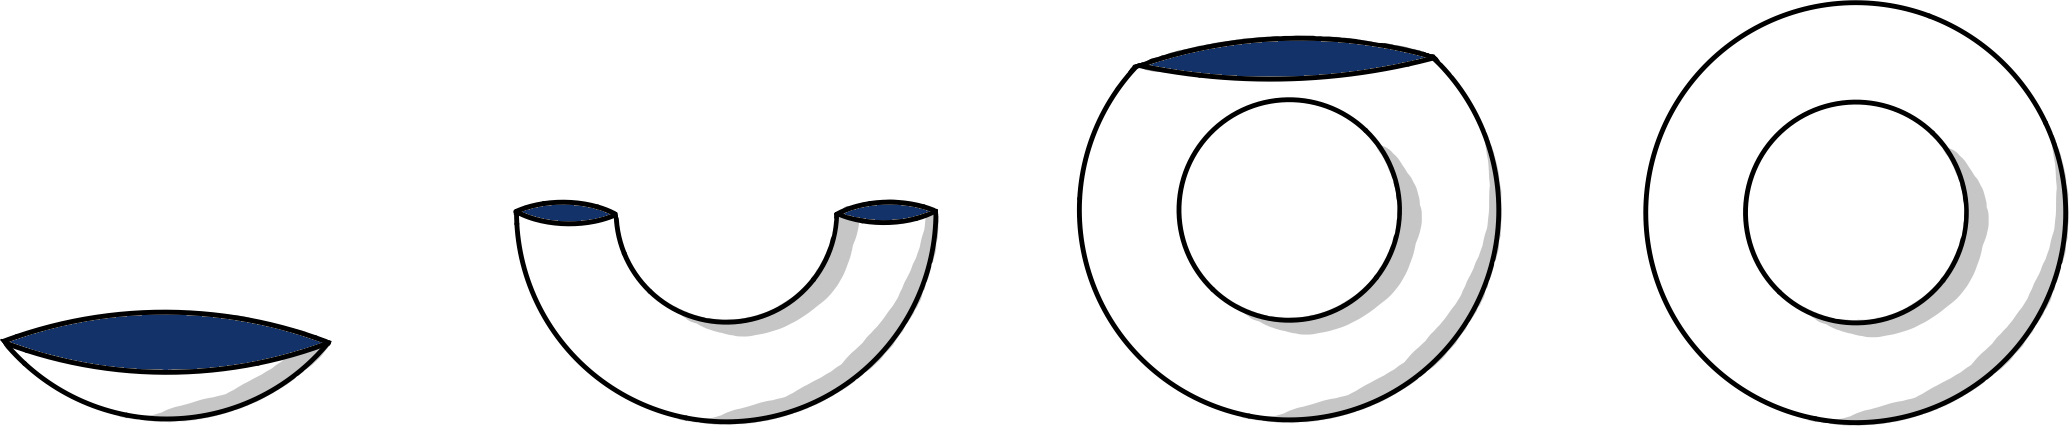
\includegraphics[width=\textwidth]{../resources/Me-Titlepage-Color.jpeg}

    \vfill
    \small

    \textit{eingereicht von}
    \hfill
    \textit{beaufsichtigt von} \\
    Jakob Dimigen
    \hfill
    Prof. Ursula Ludwig

    \vspace{2cm}

    Universität Münster \\
    \vspace{0.02cm}
    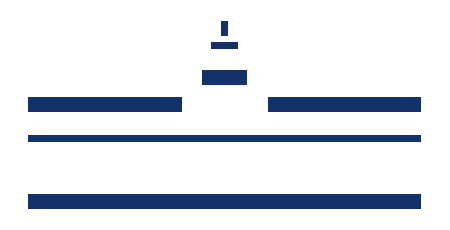
\includegraphics[width=0.2\textwidth]{../resources/WWU_Logo.png}
\end{titlepage}

\tableofcontents

\begin{abstract}
    In der Morse Theorie werden glatte Abbildungen $f \colon M \to \R$, deren kritische Punkte 
    alle nicht degeneriert sind untersucht. Anhand einer solcher Abbildungen lassen sich
    Rückschlüsse auf topologische Eigenschaften der Mannigfaltigkeit $M$ ziehen. In dieser Arbeit
    wird der \textit{Morse-Komplex} definiert, und gezeigt, dass dieser isomorph zu einem zellulären 
    Kettenkomplex ist. Dafür wird anfangs eine kurze Einführung in die Morse-Theorie gegeben und 
    grundlegende Begriffe definiert. Im zweiten Kapitel werden Morse Funktionen und Pseudo-Gradienten 
    untersucht. Im dritten Kapitel wird bewiesen, dass der Morse Komplex ein Kettenkomplex ist und 
    im letzten Kapitel wird anhand der erarbeiteten Theorie eine zelluläre Struktur auf kompakten 
    Mannigfaltigkeiten konstruiert, deren zellulärer Kettenkomplex isomorph zum Morse-Komplex ist.
    Zu guter letzt werden einige bekannte Eigenschaften der zellulären Homologie anhand der 
    Morse Homologie bewiesen. Something something
\end{abstract}

\makeheaderfancy
\setcounter{page}{1}

\chapter{Traditionelle Morse-Theorie}

Anschauliche Beispiele, vielleicht die zu den Deformations-Lemmata? Dann müsste
ich aber auch noch die Deformations-Lemmata machen.

\section{Einführung}

\subsection*{Notation}

Folgende Notationen werden benutzt:

\begin{itemize}
    \item $\isom$ für eine Vektorraum-Isomorphie oder eine Homeomorphie.
    \item $\diffeo$ für einen Diffeomorphismus.
    \item Die Tangentialräume werden immer als die Menge der Derivationen betrachtet.
    \item Um Subskripte in Subskripten weitestgehend zu vermeiden, ist ein Vektorfeld eine 
        glatte Abbildung $X \colon M \to TM$ mit $p \mapsto X(p) \in T_pM$ (anstatt $X_p$).
    \item ist $f \colon M \to \N$ eine glatte Abbiildung, dann ist die Tangentialabbildung
        von $f$ im Punkt $p$ die Abbildung $\opd f (p) \colon T_pM \to T_{f(p)}N$.
\end{itemize}

\subsection*{Vorraussetzungen}

Wir setzen vorraus, dass der Leser sich mit Mannigfaltigkeiten auskennt. Außerdem sollten 
grundlegende Begriffe der Topologie wie \textit{Homotopie}, \textit{Homotopietyp} ... \todo{...}
bekannt sein. Weiterhin sollten Grundlagen der homologischen Algebra bekannt sein, also 
Definitionen von \textit{Kettenkomplex} und \textit{Homologie}.

\subsection*{Geschichte}

Die Morse-Theorie ist zu Ehren des amerikanischen Mathematikers \textit{Marston Morse} benannt, der
grundlegende Ergebnisse zum Beispiel wie das \textit{Morse-Lemma}~\ref{satz: morse-lemma} in 
\cite{morse} schon im Jahre 1929 bewies. (Marston Morse nannte benutzte den Begriff 
\glqq Critical Point theory\grqq{})In den späten 60er Jahren untersuchte dann 
bewies.

\section{Nicht-Degeneriertheit und Index}

Dieser Abschnitt folgt dem ersten Abschnitt aus \cite{milnor}.

\begin{definition}[Kritischer Punkt]
    \label{def: kritischer Punkt}
    Sei $M$ eine glatte Mannigfaltigkeit und $f \colon M \to \R$ eine glatte Abbildung. 
    Ein \textit{kritischer Punkt} von $f$ ist ein Punkt $p \in M$, sodass $\opd f (p) = 0$.
\end{definition}

\begin{remark}
    Allgemeiner lassen sich kritische Punkte von glatten Abbildungen \\ $f \colon M \to N$ 
    definieren, siehe im Anhang Definition~\ref{anh.def: kritischer punkt}.
\end{remark}

Wir würden gerne eine Hessische Bilinearform für die Tangentialräume der Mannigfaltigkeit
definieren, allerdings ist dies ein nicht ganz einfaches Unterfangen. Wir werden am Ende
einen Begriff erhalten, der mit dem der gewohnten Hessischen Bilinearform im $\R^n$
übereinstimmt, allerdings nur für kritische Werte definiert ist.

\begin{definition}[Lie-Klammer]
    \label{def: lie-klammer}
    Es seien $X$ und $Y$ Vektorfelder auf einer glatten Mannigfaltigkeit $M$. Die 
    \textit{Lie-Klammer} ist die Abbildung 
    \begin{align*} 
        [\cdot, \cdot] \colon \VFs(M) \times \VFs(M) & \to \VFs(M) \\
        (X, Y) & \mapsto [X, Y] := XY - YX
    \end{align*}
    Wobei 
    \[ (XY - YX) (p) (f) = X(p)(Y(\cdot)(f)) - Y(p)(X(\cdot)(f)) \]
\end{definition}

\begin{remark}
    Es ist leicht nachzurechnen, dass die Lie-Klammer tatsächlich eine \\ Lie-Klammer ist,
    also dass sie folgende Eigenschaften erfüllt:
    \begin{itemize}
        \item $[\cdot, \cdot]$ ist $\R$-bilinear.
        \item $[X, Y] = -[Y, X]$
        \item $[X, [Y, Z]] + [Z, [X, Y]] + [Y, [Z, X]] = 0$
    \end{itemize}
\end{remark}

\begin{prop}
    \label{prop: lie-klammer ist null}
    Es sei $f \colon M \to \R$ glatt, $p$ ein kritischer Punkt von $f$, 
    $X, Y \in \VFs (M)$. Dann gilt:
    \[ [X, Y] (p) f = 0 \]
\end{prop}

\begin{proof}
    Es seien $(x_1, ..., x_n)$ lokale Koordinaten um $p$. Wir können ohne beschränkung
    der Allgemeinheit annehmen, dass $X = g_X \cdot \pderive{x_i}$ und 
    $Y = g_Y \cdot \pderive{x_j}$ für $g_X, g_Y \in C^{\infty} (M)$. Dann gilt:
    \begin{align*}
        \left[g_X \cdot \pderive{x_i}, g_Y \cdot \pderive{x_j}\right] (p) (f) = & 
            g_X (p) \cdot \pderive{x_i} (p) \left(g_Y \cdot \pderive[f]{x_j} \right) -
            g_Y (p) \cdot \pderive{x_j} (p) \left(g_X \cdot \pderive[f]{x_i} \right) \\
        = & g_X (p) \cdot \left( \pderive[g_Y]{x_i}(p) \cdot \pderive[f]{x_j}(p) + 
                g_Y(p) \cdot \pdderive[f]{x_j}{x_i}(p) \right) \\ 
        & - g_Y (p) \cdot \left( \pderive[g_X]{x_j}(p) \cdot \pderive[f]{x_i}(p) + 
            g_X (p) \cdot \pdderive[f]{x_i}{x_j}(p) \right) \\
        = & \; 0
    \end{align*}
    Der letzte Ausdruck ist Null wegen des Satzes von Schwarz und da $p$ ein kritischer
    Punkt von $f$ ist, also gilt $\pderive[f]{x_i}(p) = 0$.
\end{proof}

\begin{definition}[Hessische Bilinearform]
    Es sei $f \colon M \to \R$ eine glatte Abbildung, $p$ ein kritischer Punkt von $f$.
    Es seien $x, y \in T_pM$. Wähle $X, Y \in \VFs (M)$, sodass $X(p) = x$ und 
    $Y(p) = y$. Definiere nun
    \[ \opd^2 f (x, y) (p) = X(p)(Y(\cdot)f). \]
    $\opd^2 f (\cdot, \cdot) (p)$ heißt \textit{Hessische Bilinearform}. 
\end{definition}

\begin{prop}
    \label{prop: hessische ist sym bilinearform}
    $\opd^2 f (\cdot, \cdot) (p)$ hängt nicht von den gewählten Vektorfeldern $X$ und $Y$ ab 
    und ist für alle kritischen Punkte eine symmetrische Bilinearform.
\end{prop}

\begin{proof}
    Bilinearität folgt direkt aus der Definition.
    Da $p$ ein kritischer Punkt ist gilt 
    \[ \opd^2 f (x, y) (p) - \opd^2 f (y, x) (p) = [X, Y] (p) (f) = 0, \]
    die Zuordnung ist also symmetrisch. Außerdem gilt
    \[ XY f (p) = X(p) (Y(\cdot) f) = x(Y(\cdot) f), \]
    also hängt die Form nicht von $X$ ab, und wegen der Symmetrie auch nicht von $Y$.
\end{proof}

\begin{definition}[nicht-degeneriert, Index]
    \label{def: nicht-degeneriert u index}
    Es sei $f \colon M \to \R$ eine glatte Abbildung, $p$ ein kritischer Punkt von
    $f$. Wir nennen $p$ \textit{nicht degeneriert}, falls die Bilinearform 
    $\opd^2 f (\cdot, \cdot) (p)$ nicht ausgeartet ist. Der \textit{Index} eines
    nicht degenerierten kritischen Punktes ist die maximale Dimension eines
    Untervektorraumes, auf dem $\opd^2 f (\cdot, \cdot) (p)$ negativ definit ist.
\end{definition}

\begin{remark}
    Nicht-Degeneriertheit und Index lassen sich auch über lokale Koordinaten definieren,
    aber nachzurechnen, dass diese Begriffe wohldefiniert sind ist recht aufwändig.
    Trotzdem wollen wir diese Sichtweise nicht vorenthaltern:

    Es seien $\phi = (x_1, ..., x_n)$ lokale Koordinaten um den kritischen Punkt $p$. 
    Dann ist $\mathcal{B} = \left(\pderive{x_1}, ..., \pderive{x_n}\right)$ eine Basis des
    Vektorraums $T_pM$. Wir bekommen
    \[ 
        \opd^2 f \left( \pderive{x_i}, \pderive{x_j} \right) (p) 
        = \pderive{x_i}(p) \left( \pderive[f]{x_j} \right) 
        = \pdderive[f]{x_j}{x_i} (p).
    \]
    Dann ist $p$ nicht degeneriert genau dann wenn die Matrix
    \[ H^\phi_p(f) = \left( \pdderive[f]{x_i}{x_j} \right)_{1 \leq i, j \leq n} \]
    invertierbar ist. Der Index von $p$ ist dann die Anzahl der negativen Eigenwerte
    von $H^\phi_p(f)$. Der Index und die nicht-degeneriertheit hängen offensichtlich
    nicht von den gewählten Koordinaten ab, aber die Matrix $H_p^{\phi}(f)$ schon.
\end{remark}

Die Hessische Bilinearform lässt sich auch mithilfe von \textit{Zusammenhängen} für 
alle Punkte von $M$ definieren.

\begin{remark}
    Die beiden Begriffe Index und nicht-Degeneriertheit sind zentral in der Morse-Theorie 
    und werden uns über die gesamte Arbeit begleiten. Auch der nachfolgende Satz wird in 
    fast jedem Beweis genutzt:
\end{remark}

\begin{theorem}[Morse-Lemma]
    \label{satz: morse-lemma}
    Es sei $p$ ein nicht degenerierter kritischer Punkt mit Index $k$ einer glatten 
    Funktion $f \colon M \to \R$. Dann existieren lokale koordinaten 
    $\phi = (x_1, ..., x_n)$, sodass in einer Umgebung $U$ von $p$ gilt:
    \[ f = f(p) - x_1^2 - ... - x_k^2 + x_{k + 1}^2 + ... + x_n^2 \]
    und 
    \[ \varphi (p) = 0. \]
    $(U, \phi)$ heißt \textit{Morse-Karte}, und $U$ \textit{Morse-Umgebung}.
\end{theorem}

Der hier geführte Beweis für das Morse-Lemma ist in \cite{hirsch} zu finden. 
Bevor wir das Morse Lemma beweisen, benötigen wir eine Aussage aus der Linearen Algebra:

\begin{lemma}
    \label{lemma: lina lemma}
    Es sei $A = \diag(a_1, ..., a_n)$ eine diagonale $n \times n$ Matrix mit 
    Diagonaleinträgen $\pm 1$. Dann gibt es eine Umgebung $N$ von $A$ im Vektorraum der 
    symmetrischen $n \times n$ Matrizen und eine glatte Abbildung 
    $P \colon N \to GL_n(\R)$, sodass $P(A) = E_n$ und falls $P(B) = Q$, dann gilt 
    $Q^TBQ = A$.
\end{lemma}

\begin{proof}
    Betrachte zuerst den Fall $n = 1$:

    Dann ist $A = (\pm 1)$. Wähle $N = (0, 2)$ oder $N = (-2, 0)$, $P(B) := 1/\sqrt{|B|}$

    Nun $n - 1 \rightsquigarrow n$:

    Es sei $B$ eine symmetrische $n \times n$ Matrix, die nah genug an $A$ ist, sodass
    $b_{11} \neq 0$ und das selbe Vorzeichen hat wie $a_1$. Betrachte die Matrix 
    \[ T = \begin{pmatrix}
        \frac{1}{\sqrt{|b_{11}|}} & 
            - \frac{1}{\sqrt{|b_{11}|}} \cdot \frac{b_{12}}{b_{11}} & 
            - \frac{1}{\sqrt{|b_{11}|}} \cdot \frac{b_{13}}{b_{11}} & \cdots & 
            - \frac{1}{\sqrt{|b_{11}|}} \cdot \frac{b_{1n}}{b_{11}} \\
        0 & 1 & 0 & \cdots & 0 \\
        0 & 0 & 1 & \cdots & 0 \\
        \vdots & \vdots & \vdots & & \vdots \\
        0 & 0 & 0 & \cdots & 1 
    \end{pmatrix} \]
    Man rechnet nach, dass 
    \[ T^T B T = \begin{pmatrix}
        a_1 & 0 & \cdots & 0 \\
        0 & & & \\
        \vdots & & B_1 & \\
        0 & & &
    \end{pmatrix}. \]
    Die Diagonalmatrix $\diag(a_2, ..., a_n)$ ist invertierbar, und da die 
    Determinante stetig ist, ist falls $B$ nah genug an $A$ ist die symmetrische Matrix 
    $B_1$ auch invertierbar. Bemerke dass sowohl $T$ als auch $B_1$ glatte Abbildungen
    definieren. Laut Induiktionsannahme existiert eine Matrix 
    $Q_1 \in GL_n(\R)$ die glatt von $B_1$ abhängt, sodass $Q_1^T B_1 Q_1 = A_1$.
    Definiere nun $P(B) = Q$ durch $Q = TS$, wobei
    \[ S = \begin{pmatrix}
        1 & 0 & \cdots & 0 \\
        0 & & & \\
        \vdots & & Q_1 & \\
        0 & & &
    \end{pmatrix}. \]
    Dann gilt $Q^TBQ = S^T (T^T B T) S = A$.
\end{proof}

\begin{proof}[Beweis von Satz~\ref{satz: morse-lemma}]
    Es sei $U$ eine Karten Umgebung von $p$. Dann können wir ohne Beschränkung der 
    Allgemeinheit annehmen, dass $f \colon \R^n \to \R$, $p = 0$ und $f(0) = 0$.
    Außerdem können wir mithilfe eines Korrdinatenwechsels annehmen, dass 
    \[ A = H_0(f) \]
    eine Diagonalmatrix mit ausschließlich Diagonaleinträgen $\pm 1$ hat, denn da $p$
    nicht degeneriert ist ist $A$ invertierbar. 
    \begin{claim*}
        Es existiert eine glatte Abbildung $x \mapsto B_x$ von $M$ in die symmetrischen
        $n \times n$ Matrizen, sodass für $B_x = (b_{ij}(x))_{ij}$ gilt 
        \[ f(x) = \sum_{i, j = 1}^n b_{ij}(x) x_i x_j , \]
        und sodass $B_0 = A$. 
    \end{claim*}
    \begin{smallproof}
        Da $f(0) = 0$ bekommen wir mit dem Fundamentalsatz der 
        Differenzial - und Integralrechnung: 
        \begin{align*}
            f(x) = & f(x) - f(0) \\
            = & \int_0^1 \derive[f (tx)]{t} \opd t \\
            = & \int_0^1 \sum_{i = 1}^n \pderive[f]{x_i}(tx) x_i \opd t \\
            = & \sum_{i = 1}^n \left( \int_0^1 \pderive[f]{x_i}(tx) \opd t \right) x_i
        \end{align*}
        Da $p = 0$ ein kritischer Punkt ist, gilt $\pderive[f]{x_i}(0) = 0$ für alle 
        $i$. Mit dem selben Argument sehen wir dann, dass
        \[ \pderive[f]{x_i}(tx) = 
        \sum_{j = 1}^n \left( \int_0^1 \pdderive[f]{x_i}{x_j}(stx) \opd s \right) x_j . \]
        Dann gilt 
        \[ f(x) = 
            \sum_{i, j = 1}^n 
            \left( \int_0^1 \int_0^1 \pdderive[f]{x_i}{x_j} \opd s \opd t \right) 
            x_i x_j 
        . \]
        Setze also 
        \[ b_{ij}(x) = \int_0^1 \int_0^1 \pdderive[f]{x_i}{x_j} \opd s \opd t . \]
        Dann gilt schon $B_0  = A$, und die Abbilfungen $b_{ij}$ sind glatt, also 
        auch $x \mapsto B_ x$.
    \end{smallproof}
    Wir dürfen nun das vorherige Lemma~\ref{lemma: lina lemma} anwenden:

    Sei $P \colon N \to GL_n(\R)$ eine Abbildung wie in~\ref{lemma: lina lemma}.
    Setze $P(B_x) := Q_x$ Definiere nun eine glatte Abbildung $\phi \colon U \to \R^n$
    durch $\phi (x) = Q_x^{-1}x$ in einer Umgebung von $0$. Wir rechnen nach, dass 
    $\opd \phi (0) \colon \R^n \to \R^n$ die Identität ist:

    Schreibe $Q_x^{-1} = (q_{ij}(x))_{ij}$. Dann
    \[ \phi(x) = \left( 
        \sum_{k = 1}^n q_{1k}(x) x_k, \cdots , \sum_{k = 1}^n q_{nk}(x) x_k
        \right)
    \]
    Also 
    \begin{align*}
        \pderive[\phi_i]{x_j} (x) 
            = & \pderive{x_j} \left( \sum_{k = 1}^n q_{ik} (x) x_k \right) \\
        = & \sum_{k = 1}^n \left( 
            \pderive[q_{ik}]{x_j}(x) x_k + q_{ik}(x) \delta_{ki}
        \right)
    , \end{align*}
    Wobei $\delta_{ki}$ das Kronecker Delta ist. Setzen wir also $0$  in $\phi$ ein
    bekommen wir
    \[ \pderive[\phi_i]{x_j}(0) = q_{ij}(0). \]
    Das Differential von $\phi$ in $0$ ist also gegeben durch
    \[ Q_0^{-1} = P(B_0)^{-1} = P(A)^{-1} = E_n . \]
    Das differential an der Stelle $0$ ist also invertierbar, und dann können wir mit dem 
    Satz über die Umkehrfunktion annehmen, dass $U$ klein genug ist, sodass $\phi$ 
    eingeschräkt aufs Bild ein Diffeomorphismus ist. 
    Dann ist $\phi$ eine Karte um $0$. Setze $(y_1, ..., y_n) := \phi$, dann gilt 
    \begin{align*}
        f(x) = & x^T B_x x \\
        = & (Q_x \phi(x))^T B_x (Q_x \phi(x)) \\
        = & \phi(x)^T (Q_x^T B_x Q_x) \phi(x) \\
        = & \phi(x)^T A \phi(x) \\
        = & \sum_{i = 1}^n a_{ii} y_i(x)^2
    . \end{align*}
    Das entspricht genau der gewünschten Form.
\end{proof}

\begin{corollary}
    Nicht-degenerierte kritische Punkte sind isoliert.
\end{corollary}


\chapter{Morse-Funktionen und Pseudo-Gradienten}

Das Ziel dieses Kapitels ist es, Morse-Funktionen und Pseudo-Gradienten zu
definieren und ihre \todo{allgegen- wertigkeit ist nicht so ein schönes Wort}
\textit{allgegenwertigkeit} zu zeigen. Ein weiteres wichtiges Ergebnis ist
das \textit{Morse-Lemma}.

\section{Morse-Funktionen}

In diesem Abschnitt untersuchen wir \textit{Morse-Funktionen}:

\begin{definition}[Morse-Funktion]
    \label{satz: morse-funktion}
    Eine \textit{Morse-Funktion} auf einer glatten Mannigfaltigkeit $M$ ist eine glatte Funktion
    $f \colon M \to \R$, deren kritische Punkte alle nicht degeneriert sind.
\end{definition}

Insbesondere zeigen wir, dass Morse Funktionen nichts besonderes sind. Dafür zeigen wir, dass für 
eine Untermannigfaltigkeit $M \subseteq \R^n$ und einen Punkt $p \in \R^n$ die Abbildung
$x \mapsto \| x - p \|^2$ nur für $p$, die so gennanten \textit{Brennpunkte}
sind, keine Morse Funktion ist.

\begin{definition}[Normalenbündel]
    \label{def: normalenbuendel}
    Es sei $M \subseteq \R^n$ eine Untermannigfaltigkeit von $\R^n$. Das Normalenbündel ist die 
    Menge
    \[ NM = \{ (x, v) \in M \times \R^n : v \perp T_xM \} . \]
    Wir betrachten hier $T_xM \subseteq T_x\R^n \isom \R^n$ via der Basis 
    $\left( \del / \del x_i \right)$, wobei $x_i$ die Achsen des $\R^n$ sind.
\end{definition}

\begin{prop}
    \label{prop: NM ist untermannigfaltigkeit}
    Das Normalenbündel $NM$ ist eine $n$-dimensionale Untermannigfaltigkeit von $M \times \R^n$.
\end{prop}

\begin{proof}
    Es sei $x \in M$. Dann existiert eine Umgebung $U \subseteq \R^n$ von $x$, eine Umgebung 
    $\Omega \subseteq \R^d$ von $0$ und eine Immersion 
    \begin{align*}
        h \colon \Omega \longto & \R^n \\
        (u_1, \dots, u_d) \; \longmapsto & \; x(u_1, \dots, u_d)
    \end{align*}
    die ein Diffeomorphismus $h \colon \Omega \to U \cap M$ ist. Das orthogonale Komplement 
    von $T_xM$ in $\R^n$ hat Dimension $n - d$. Es sei also 
    $(v_1(x), ..., v_{n-d}(x))$ eine Basis von $(T_xM)^{\perp}$. Dann ist 
    \[ (u_1, ..., u_d, t_1, ..., t_{n - d}) \longmapsto 
        \left(x(u_1, ..., u_n), \sum_{k = 1}^{n - d} t_k \cdot v_k(u_1, ..., u_d)\right) \]
    eine lokale Parametrisierung von $NM$ als Untermannigfaltigkeit von $M \times \R^n$.
\end{proof}

\begin{definition}[Brennpunkt]
    \label{def: brennpunkt}
    Es sei $M \subseteq \R^n$ eine Untermannigfaltigkeit von $\R^n$. Es sei $E \colon NM \to R^n$ 
    mit $E (x, v) = x + v$. Ein \textit{Brennpunkt} von $M$ ist ein kriticher Wert von $E$.
\end{definition}

\begin{remark}
    Aus dem Satz von Sard folgt, dass die Menge der Brennpunkte eine Nullmenge ist.
    Intuitiv sind die Brennpunkte einer Untermannigfaltigkeit die Punkte im $\R^n$, an denen sich
    die Normalen von nahe aneinanderliegenden Punkten schneiden.
\end{remark}

\begin{lemma}
    \label{lemma: char. von Brennpunkten}
    Es sei $M \subseteq \R^n$ eine Untermannigfaltigkeit von $\R^n$ $x \in M$ und $M$ in einer 
    Umgebung von $x$ und $NM$ parametriesiert wie im Beweis von 
    Proposition~\ref{prop: NM ist untermannigfaltigkeit}. Dann ist $p = x + v$ genau dann ein
    Brennpunkt von $M$, wenn die Matrix 
    \[
        \left( \left\langle \pderive[x]{u_j}, \pderive[x]{u_i} \right\rangle - 
        \left\langle v , \pdderive[x]{u_i}{u_j} \right\rangle \right)_{ij}
    \]
    nicht invertierbar ist.
\end{lemma}

\begin{proof}
    Wir haben partielle Ableitungen
    \[ \pderive[e]{u_i} = \pderive[x]{u_i} + \sum_{k = 1}^{n - d} t_k \pderive[v_k]{u_i} \]
    und 
    \[ \pderive[E]{t_j} = v_j \]
    Nun ein kleines Ergebnis aus der Linearen Algebra:

    sind $v_1, ..., v_n, u_1, ..., u_n \in \R^n$ und $u_1, ..., u_n$ linear unabhängig, 
    dann ist
    \[ (v_1 \; ... \; v_n)^T \cdot (u_1 \; ... \; u_n) = (\langle v_i, u_j \rangle)_{ij} , \]
    Also 
    \[ \rank (v_1 ... v_n) = \rank (\langle v_i, u_j \rangle)_{ij} . \]

    Die Vektoren $ \pderive[x]{u_1}, ..., \pderive[x]{u_d}, v_1, ..., v_{n - d}$ sind linear
    unabhängig. Außerdem ist $\pderive[x]{u_l}$ orthogonal zu $v_k$, also hat die Matrix mit 
    Einträgen die Skalarprodukte dieser linear unabhängigen Vektoren mit den obigen partiellen
    Ableitungen von $E$ die Form 
    \[
        \begin{pmatrix}
            \left( \left\langle \pderive[x]{u_i}, \pderive[x]{u_j} \right\rangle + 
                \sum_{k = 1}^{n - d} t_k 
                \left\langle \pderive[v_k]{u_i} , \pderive[x]{u_j} \right\rangle \right)_{ij} &
            \left( \sum_{k = 1}^{n - d} 
                \left\langle \pderive[v_k]{u_i}, v_j \right\rangle \right)_{ij} \\
            0 & E_{n - d}
        \end{pmatrix}
    \]
    Diese Matrix hat Rang $< n$ genau dann, wenn 
    \[ \rank \left( \left\langle \pderive[x]{u_i}, \pderive[x]{u_j} \right\rangle + 
        \sum_{k = 1}^{n - d} t_k 
        \left\langle \pderive[v_k]{u_i} , \pderive[x]{u_j} \right\rangle \right)_{ij} < d 
    , \]
    Aber da $v_k$ und $\pderive[x]{u_j}$ orthogonal aufeinander stehen gilt 
    \[ 
        0 = \pderive{u_i} \left\langle v_k, \pderive[x]{u_j} \right\rangle
        = \left\langle \pderive[v_k]{u_j}, \pderive[x]{u_i} \right\rangle 
        + \left\langle v_k, \pdderive[x]{u_i}{u_j} \right\rangle
    \]
    Also 
    \begin{align*}
        \left\langle \pderive[x]{u_i}, \pderive[x]{u_j} \right\rangle + 
                \sum_{k = 1}^{n - d} t_k 
                \left\langle \pderive[v_k]{u_i} , \pderive[x]{u_j} \right\rangle
        = & \left\langle \pderive[x]{u_i}, \pderive[x]{u_j} \right\rangle - 
        \sum_{k = 1}^{n - d} t_k 
        \left\langle v_k , \pdderive[x]{u_i}{u_j} \right\rangle \\
        = & \left\langle \pderive[x]{u_i}, \pderive[x]{u_j} \right\rangle - 
        \left\langle v , \pdderive[x]{u_i}{u_j} \right\rangle
    \end{align*}
    Es folgt die Behauptung.
\end{proof}

\begin{prop}
    \label{prop: existenz morse-funktionen}
    Es sei $M \subseteq \R^n$ eine Untermannigfaltikgeit. Für fast jeden Punkt in $\R^n$ ist
    die Funktion
    \begin{align*}
        f_p \colon M & \longrightarrow \R \\
        x & \longmapsto \| x - p \|^2
    \end{align*}
    eine Morse-Funktion.
\end{prop}

\begin{proof}
    Offensichtlich ist $f_p$ glatt. $x \in M$ ist genau dann ein kritischer Punkt von $f_p$, wenn
    $T_xM \perp (x - p)$, denn das differential von $f_p$ erweitert auf $\R^n$ ist
    \[ \opd f_p (x) = 2 (x - p). \]
    Also gilt
    \[ \opd f_p (x) (v) = \langle 2 (x - p), v \rangle . \]
    $x \in M$ ist folglich genau dann ein kritischer Punkt von $f_p$, wenn $T_xM$ orthogonal 
    zu $(x - p)$ ist.

    Bemerke, dass für eine Abbildung $f \colon \R^n \to \R$ mit $f = \langle \phi_1, \phi_2 \rangle$,
    $\phi_1, \phi_2 \colon \R^n \to \R^n$ und eine Derivation $X_p$ gilt 
    \[ X_p (f) = \langle X_p(\phi_1), \phi_2 \rangle + \langle \phi_1, X_p(\phi_2) \rangle.  \]
    Sei nun $x \in M$. Dann existiert eine Umgebung $U \subseteq \R^n$ von $x$, eine Umgebung 
    $\Omega \subseteq \R^d$ von $0$ und eine Immersion 
    \[ h \colon \Omega \longto \R^n , \]
    die ein Diffeomorphismus $h \colon \Omega \to U \cap M$ ist.
    Schreibe
    \[ h(u_1, ..., u_n) = x(u_1, ..., u_n). \]
    Dann bekommen wir die partiellen Ableitungen
    \[ 
        \pderive[f_p]{u_i} = \sum_{k = 1}^n \pderive[f_p]{x_k} \cdot \pderive[x_k]{u_i} 
        = \langle 2(x - p), \pderive[x]{u_i} \rangle 
    \]
    und 
    \[ 
        \pdderive[f_p]{u_i}{u_j} = 
            2 \left( \left\langle \pderive[x]{u_j}, \pderive[x]{u_i} \right\rangle + 
            \left\langle x - p , \pdderive[x]{u_i}{u_j} \right\rangle \right) 
    . \]
    
    Also hat nach Lemma~\ref{lemma: char. von Brennpunkten} $f_p$ in einer Umgebung von $x$ genau 
    dann nicht-degenerierte kritische Punkte, wenn $f_p$ ein Brennpunkt von $M$ ist. Mit der 
    Bemerkung nach der Definition von Brennpunkten~\ref{def: brennpunkt} folgt dann direkt die 
    Behauptung.
\end{proof}

\begin{remark}
    Mit dem Einbettungssatz von Whitney folgt dann direkt, dass es auf jeder Mannigfaltigkeit 
    $M$ viele Morse-Funktionen gibt. Wir können sogar noch eine stärkere Aussage beweisen:
\end{remark}

\begin{theorem}
    \label{satz: morse-approximation}
    Es sei $M$ eine Mannigfaltigkeit, $f \colon M \to \R$ glatt. Dann kann $f$ in jeder kompakten
    Teilmenge $K$ beliebig gut von einer Morse Funktion approximirt werden, also für jedes 
    $\eps > 0$ existiert eine Morse Funktion $g \colon K \to \R$, sodass 
    \[ \| \, f - g \, \|_{\infty} < \eps . \]
\end{theorem}

\begin{proof}
    Wir wählen eine Einbettung $h' \colon M \to \R^{n - 1}$. Dann ist 
    \[ h \colon M \longto \R^n \; ; \; h(x) = (f(x), h'(x)) \]
    eine Einbettung von $M$ in $\R^n$. Seien $c, \eps_1, \dots, \eps_n > 0$, sodass für \\
    $p = (c - \eps_1, \eps_2, \dots, \eps_n)$ die Funktion $f_p$ eine Morse Funktion ist.
    Setze nun 
    \[ g(x) = \frac{f_p(x) - c^2}{2c} . \]
    $g$ ist offensichtlich eine Morse-Funktion. Wir rechnen:
    \begin{align*}
        g(x) = & \frac{1}{2c} \left( (f(x) + c - \eps_1)^2 + (h_1(x) - \eps_2)^2 
            + \dots + (h_{n-1}(x) - \eps_n)^2 - c^2 \right) \\
        = & f(x) + \frac{f(x)^2 + \sum h_i(x)^2}{2c} - \frac{\eps_1 f(x) 
            + \sum \eps_i h_{i - 1}(x)}{c} + \sum \eps_i^2 - \eps_1
    \end{align*}
    Man kann nun $c$ beliebig groß und $\eps_1, \dots, \eps_n$ beliebig klein wählen,
    sodass $g$ beliebig nah an $f$ ist.
\end{proof}

\begin{remark}
    Die meiste Zeit werden wir uns in dieser Arbeit kompakte Mannigfaltigkeiten untersuchen,
    auf solchen kann jede glatte Funktion sogar global mit einer Morse Funktion approximieren.
\end{remark}

section{Vektorfelder und Pseudo-Gradienten}

Wir untersuchen erst ein Paar Eigenschaften von Vektorfeldern.

\begin{definition}[Flusslinie]
    \label{def: flussliene}
    Es sei $I \subseteq \R$ ein Intervall, $M$ eine glatte Mannigfaltigkeit und  
    $\gamma \colon I  \to M$ ein glatter Weg. Dann definiere für $t_0 \in \R$
    \[ \derive[\gamma]{t} (t_0) := 
        \opd \gamma (t_0) \left( \pderive{t} \right) \in T_{\gamma(t_0)}M \]
    wobei $\pderive{t}$ das von der Indentität auf $\R$ induziertze Element in $T_t\R$ ist.

    Es sei $X \in \VFs (M)$ ein Vektorfeld auf $M$. $\gamma$ heißt Flusslinie von $X$
    falls für alle $t_0 \in \R$ gilt: 
    \[ \derive[\gamma]{t}(t_0) = X(\gamma(t_0)) . \]
\end{definition}

\begin{definition}[1-Parameter Gruppe aus Diffeomorphismen]
    \label{def: 1-parameter gruppe aus diffeos}
    Es sei $M$ eine glatte Mannigfaltigkeit. Eine 
    \textit{1-Parameter Gruppe aus Diffeomorphismen} ist eine glatte Abbildung
    \begin{align*}
        \phi \colon \R \times M \longto & \; M \\
        (t, p) \longmapsto & \; \phi_t(p)
    \end{align*}
    sodass gelten: 
    \begin{itemize}
        \item Für alle $s, t \in \R$ gilt $\phi_{s + t} = \phi_s \circ \phi_t$ und
        \item $\phi_0 = \id_{M}$.
    \end{itemize}

    Für eine 1-Parameter Gruppe aus Diffeomorphismen $\phi$ schreiben wir 
    \[ \varphi_{\bullet}(p): \R \to M ; t \mapsto \varphi_t(p) . \]

    Es sei $X \in \VFs (M)$. Eine 1-Parameter Gruppe aus Diffeomorphismen $\phi$ heißt 
    \textit{von $X$ erzeugt}, falls für alle $p \in M$ gilt:
    \[ X(p) = \derive[\phi_{\bullet}(p)]{t}(0) \]
\end{definition}

\begin{remark}
    Wie der Name suggestiert, ist für jedes $t \in \R$ $\phi_t$ ein 
    Diffeomorphismus: Das Inverse von $\phi_t$ ist $\phi_{-t}$.

    Ist außerdem $\phi$ eine von einem Vektorfeld $X$ erzeugte 1-Parameter Gruppe aus 
    Diffeomorphismen, dann sind $\phi_{\bullet}(p)$ Flusslinien von $X$:
    \begin{align*}
        X(\varphi_{t_0}(p)) 
        & = \derive[\varphi_{\bullet}(\varphi_{t_0}(p))]{t}(0)
        = \opd \varphi_{\bullet} (0) (\varphi_{t_0}(p)) \left(\derive{t}\right) \\
        & = \opd (\varphi_{t_0 + \bullet}(p)) (0) \left(\derive{t}\right)
        = \opd (\varphi_{\bullet}(p)) (t_0) \cdot \opd (t_0 + \id_{\R}) (0) \left(\derive{t}\right) \\
        & = \opd (\varphi_{\bullet}(p)) (t_0) \left(\derive{t}\right)
        = \opd (\varphi_{\bullet}(p)) (t_0) \left(\derive{t}\right) \\
        & = \derive[\varphi_{\bullet}(p)]{t}(t_0)
    \end{align*}
\end{remark}

\begin{prop}
    \label{prop: kompaktes VF generiert 1-param. grp.}
    Es sei $M$ eine glatte Mannigfaltigkeit, $X \in \VFs (M)$ mit kompaktem Träger. Dann 
    generiert $X$ eine eindeutige 1-Parameter Gruppe aus Diffeomorphismen.
\end{prop}

\begin{proof}
    Für jeden Punkt $p \in M$ existiert eine Karten-Ungebung $(U_p, \phi_p)$. In dieser
    Umgebung hat das Anfangswertproblem
    \[ \derive[\gamma]{t} = X (\gamma) \; , \; \gamma(0) = p \]
    eine eindeutige Lösung in einem Intervall $[-\eps_p, \eps_p]$. Diese Lösung 
    $\gamma$ hängt glatt vom Anfangswert ab. Wir schreiben
    $\phi_{\bullet}(p) := \gamma$. In dieser Umgebung gilt schon \\ 
    $\phi_{t + s} = \phi_t \circ \phi_s$, solange $t, s, t + s \in [-\eps_p, \eps_p]$. 
    Da $\supp \, X$ kompakt ist existiert eine endliche Menge ${p_1, \dots, p_k}$, 
    sodass $\supp \, X \subseteq \bigcup_i U_{p_i}$. Es sei $\eps$ das Minimum der 
    $\eps_{p_i}$. Setze $\phi_t(p) = p$ für alle $p$ nicht im Träger von $X$. Wir haben nun 
    fast einen Kandidaten für die von $X$ generierte 1-Parameter Gruppe aus Diffeomorphismen;
    $\phi_t(p)$ ist definiert für alle $p \in M$ und $t \in [-\eps, \eps]$. Wir müssen also nur 
    noch einen Kandidaten für $\phi_t(p)$ finden, falls $|t| \geq \eps$.

    Wir können jede Zahl $t \in \R$ schreiben als $t = m \cdot \sfrac{\eps}{2} + r$ mit 
    $0 \leq r < \sfrac{\eps}{2}$ und $m \in \Z$. Sei nun zuerst $t \geq 0$, dann ist $m \geq 0$.
    Setze für alle $p \in M$ 
    \[ \phi_t(p) 
        := \phi_{\sfrac{\eps}{2}} \circ \dots \circ \phi_{\sfrac{\eps}{2}} \circ \phi_r , \] 
    Wobei wir $\phi_{\sfrac{\eps}{2}}$ $|m|$ mal anwenden. Falls $t < 0$ ersetze $\sfrac{\eps}{2}$
    mit $- \sfrac{\eps}{2}$. 
\end{proof}

\begin{remark}
    Falls $M$ eine kompakte Mannigfaltigkeit ist, dann generieren alle Vektorfelder eindeutige 
    1-Parametergruppen aus Diffeomorphismen.
\end{remark}

\begin{definition}[Riemannsche Metrik]
    \label{def: riemannsche metrik}
    Es sei $M$ eine Mannigfaltigkeit. Es sei 
    \[ g_p \colon T_pM \times T_pM \longto T_pM \]
    ein Skalarprodukt für jedes $p \in M$, sodass für alle $X, Y \in \VFs (M)$ die Abbildung 
    \[ p \longmapsto g_p(X(p), Y(p)) \]
    glatt ist. Dann heißt $g$ \textit{Riemmannsche Metrik} auf $M$. Wir schreiben für 
    $x, y \in T_pM$ 
    \[ \langle x, y \rangle := g_p(x, y) \text{ und } \| x \| := \sqrt{g_p(x, x)} . \]
\end{definition}

\begin{remark}
    Man kann zeigen, dass alle Mannigfaltigkeiten eine Riemannsche Metrik besitzen.
\end{remark}

\begin{definition}[Gradient]
    \label{def: gradient}
    Es sei $M$ eine glatte Mannigfaltigkeit, $f \colon M \to \R$ eine glatte Abbilding. Dann 
    ist der Gradient von $f$ das eindeutige Vektorfeld $\grad f$, sodass für alle $X \in \VFs (M)$
    gilt 
    \[ \langle X , \grad f \rangle = \opd f X . \]
\end{definition}

\begin{definition}[Pseudo-Gradient]
    \label{def: pseudo-gradient}
    Es sei $M$ eine Mannigfaltigkeit, $f \colon M \to \R$ eine glatte Funktion. $X \in \VFs (M)$
    heißt \textit{Pseudo-Gradient} oder \textit{Pseudo-Gradientenfeld} von $f$, falls gelten:
    \begin{itemize}
        \item $\opd f (p) (X(p)) \leq 0$ für alle $p \in M$, mit Gleichheit genau dann wenn 
            $p$ ein kritischer Punkt von $f$ ist.
        \item Für jeden kritischen Punkt $p$ von $f$ existiert eine Morse-Umgebung 
            $(U_p, \phi_p)$, in der $X (q) = - \opd (\phi_p^{-1}) (q) \cdot \grad (f \circ \phi_p^{-1})$.
    \end{itemize}
\end{definition}

\begin{prop}
    Es sei $M$ eine Mannigfaltigkeit und $f \colon M \to \R$ eine Morse-Funktion. 
    Dann existiert ein Pseudo-Gradientenfeld von $f$.
\end{prop}

\begin{proof}
    Da $M$ zweitabzählbar ist und die kritischen Punkte isoliert, ist die Menge der kritischen
    punkte ${p_i}_{i \in I'}$ abzählbar. Seien dann ${(U_i, \phi_i)}_{i \in I'}$ Karten-Umgebungen
    von den kritischen Punkten, sodass in diesen Umgebungen $f$ die Form hat wie im 
    Morse-Lemma~\ref{satz: morse-lemma}. Ergänze ${(U_i, \phi_i)}_{i \in I'}$ zu einem Atlas 
    ${(U_i, \phi_i)}_{i \in I}$, sodass jeder kritische Punkt $p_i$ nur in $U_i$ enthalten ist.
    definiere nun die Vektorfelder
    \[ X_i (p) := \opd (\phi_i) (p) \circ \grad (f \circ \phi_i^{-1}) (\phi_i(p)) \]
    auf $\phi_i(U_i)$. Setze nun
    \[ \tilde{X_i}(p) = \begin{cases}
        \lambda_i (p) \cdot X_i(p) & \text{ falls } p \in \phi_i(U) \\
        0 & \text{ sonst }
    \end{cases} . \]
    Per Definition gilt schon $\opd f (p) (X_i(p)) \leq 0$ für alle $p \in M$ und $i \in I$.
    Nun wähle eine Partition der 1 $(\lambda_i)_{i \in I}$ über $(U_i)_{i \in I}$. Dann setze
    \[ X := \sum_{i \in I} \tilde{X_i}(p) . \]
    Falls $p_i$ ein kritischer Punkt von $M$ ist, dann ist $\tilde{X_j}(p) = 0$ 
    für alle $j \neq i$. Also ist 
    \[ X(p) = \tilde{X_i}(p) = 0 . \]
\end{proof}
\section{Topologische Eigenschaften anhand kritischer Punkte}

Wir wollen die beiden Deformations-Lemmata beweisen, die eine Verbindung zwischen den topologischen
Eingeschaften einer Mannigfaltigkeit und den kritischen Punkten einer Morse Funktion herstellt.
Ist $f \colon M \to \R$ eine glatte Abbildung, dann ist die Subniveaumenge von $f$ bezüglich 
einer reellen Zahl $c$ die Menge $M^c := f^{-1}(- \infty, c]$. Sind $a < b$ reelle Zahlen, dann
stellen die Deformationslemmata die Topologien von $M^a$ und $M^b$ in Relation: Das erste beschreibt, 
was passiert \textit{wenn kein} kritischer Wert überschritten wird, und das zweite beschreibt, was 
passiert \textit{wenn ein} kritischer Wert überschritten wird. Die Beweise folgen Milnors Buch 
\cite{morse}.

\begin{theorem}[Erstes Deformationslemma]
    \label{satz: erstes deformationslemma}
    Es sei $M$ eine glatte Mannigfaltigkeit und $f: M \rightarrow \R$ eine
    glatte Abbildung. Hat $f$ keine kritischen Werte im Intervall $[a, b]$ und 
    ist $f^{-1}[a, b]$ kompakt, so existiert ein Diffeomorphismus 
    $M^a \rightarrow M^b$, und $M^a$ ist ein Deformationsretrakt von $M^b$.
\end{theorem}

Die Idee des Beweises ist es, $M^a$ entlang der Richtung, in die $f$ am stärksten
steigt, also entlang des Gradientenfeldes mit einem Diffeomorphismus $\varphi$ 
"nach oben zu ziehen", bis $\varphi(f^{-1}(a)) = f^{-1}(b)$.

\begin{proof}
    Es existiert eine kompakte Umgebung $K \in M$ von $f^{-1}[a, b]$, in der keine kritischen Punkte 
    enthalten sind, das folgt zum Beispiel aus Whitneys Einbettungssatz und dem Satz von Heine-Borel. 
    Sei $\rho: M \to \R$ eine glatte, positive Funktion, sodass
    \[ \rho(p) = 1 / \langle \grad f, \grad f \rangle \]
    für alle $p \in f^{-1}[a, b]$ und die außerhalb von $K$ verschwindet und für
    die für alle $p \in K$, die keine kritischen Punkte sind, gilt: 
    \[ 0 \leq \rho(p) \leq 1 / \langle \grad f, \grad f \rangle \]
    Bemerke dass $\rho$ innerhalb von $K$ wohldefiniert ist, da sich keine kritischen Punkte in $K$ 
    befinden. Definiere ein Vektorfeld $X$ durch
    \[ X(p) = \rho(p) \cdot \grad f (p) \]
    Dann hat $X$ kompakten Träger, erfüllt also die Vorraussetzungen von 
    Lemma~\ref{prop: kompaktes VF generiert 1-param. grp.}. Sei also $\varphi$ die
    einzigartige 1-Parameter Gruppe aus Diffeomorphismen, die von $X$ generiert
    wird. 
    Wir bekommen für jedes $p \in M$ eine Abbildung 
    $f \circ \varphi_{\bullet}(p): \R \to \R$.
    
    \begin{claim*} 
        Für alle $p \in M$, $t_0 \in \R$ und $q = \varphi_{t_0}(q)$
        ist $\derive{t} f \circ \varphi_{\bullet}(p) (t_0) \in [0, 1]$ und falls 
        $f(\varphi_t(q)) \in [a, b]$ gilt sogar $\derive{t} f \circ \varphi_{\bullet}(q) (t_0) = 1$.
    \end{claim*}

    \begin{smallproof}
        Für $q = \varphi_{t_0}(p)$:
        \begin{align*}
            \derive{t} f \circ \varphi_{t_0}(p)
            & = \opd f (\varphi_{t_0}(p)) \cdot \opd \varphi_{\bullet}(p) (t_0) 
                \left( \derive{t} \right)
            = \opd f (q) \cdot X(q) \\
            & = \langle X(q), \grad f (q) \rangle 
            = \rho(q) \langle \grad f (q), \grad f (q) \rangle \in [0, 1]
        \end{align*}
        $f \circ \varphi_{\bullet}(p)$ ist also monoton wachsend für alle $p \in M$.
        Falls sogar $f(\varphi_p(t_0)) \in [a, b]$, dann gilt
        \[ \frac{d}{dt} f \circ \varphi^p (t_0) = 1 \]
    \end{smallproof}

    Man zeigt dann leicht, dass für $p \in f^{-1}(a)$, $t_0 \in [0, b-a]$ gilt 
    $f(\varphi_{t_0}(p)) \in [a, b]$.

    Dann ist für $p \in f^{-1}(a)$ die Abbildung $f \circ \phi_{bullet}(p)$ im Intervall $[0, b - a]$
    linear mit Steigung $1$ und es gilt 

    \[ f(\varphi_{b - a}(p)) = f(\varphi_{0}(p)) + (b - a) = b \]
    Genauso für $q \in f^{-1}(b)$: $f(\varphi_{a - b}(q)) = a$, also 
    $\varphi_{b - a}(f^{-1}(a)) = f^{-1}(b)$.

    Dann haben wir $\varphi_{b - a} (M^a) = M^b$, also ist $\varphi_{b - a}|_{M^a}$ ein 
    Diffeomorphismus zwischen $M^a$ und $M^b$. 

    Betrachte nun $r: M^b \times \R \to M^b$,
    \[  
        r(p, t) = \begin{cases}
            p & \text{ falls } f(p) \leq a \\
            \varphi_{t(a - f(p))}(p) & \text{ falls } a \leq f(p) \leq b 
        \end{cases}
    \]

    $r$ ist stetig, $r(\cdot, 0)$ ist die Identität auf $M^b$, 
    $r(\cdot, 1)|_{M^a}$ ist die Identität auf $M^a$ und 
    $r(1, M^b) \subseteq M^a$, also ist $M^a$ ein Deformationsretrakt von $M^b$.
\end{proof}

\begin{theorem}[Zweites Deformations-Lemma]
    \label{satz: zweites deformationslemma}
    Es sei $M$ eine glatte Mannigfaltigkeit, $f: M \rightarrow \R$ eine glatte
    Abbildung und $p$ ein nicht-degenerierter kritischer Punkt mit Index 
    $k$. Sei $c := f(p)$ und $\varepsilon \geq 0$, sd. 
    $f^{-1}[c - \varepsilon, c + \varepsilon]$ kompakt ist und außer $p$ keine 
    weiteren kritischen Punkte von $f$ beinhaltet. Dann hat $M^{c-\varepsilon}$
    denselben Homotopietypen wie $M^{c - \varepsilon} \cup e^k$.
\end{theorem}

\begin{proof}
    Die Idee für den Beweis ist, sich eine neue Funktion $F: M \to \R$ zu definieren,
    die Außerhalb von einer kleinen Umgebung von $p$ $f$ entspricht und in der 
    Umgebung etwas kleiner ist. Dann bekommen wir die folgende Situation:

    \begin{figure}[H]
        \centering
        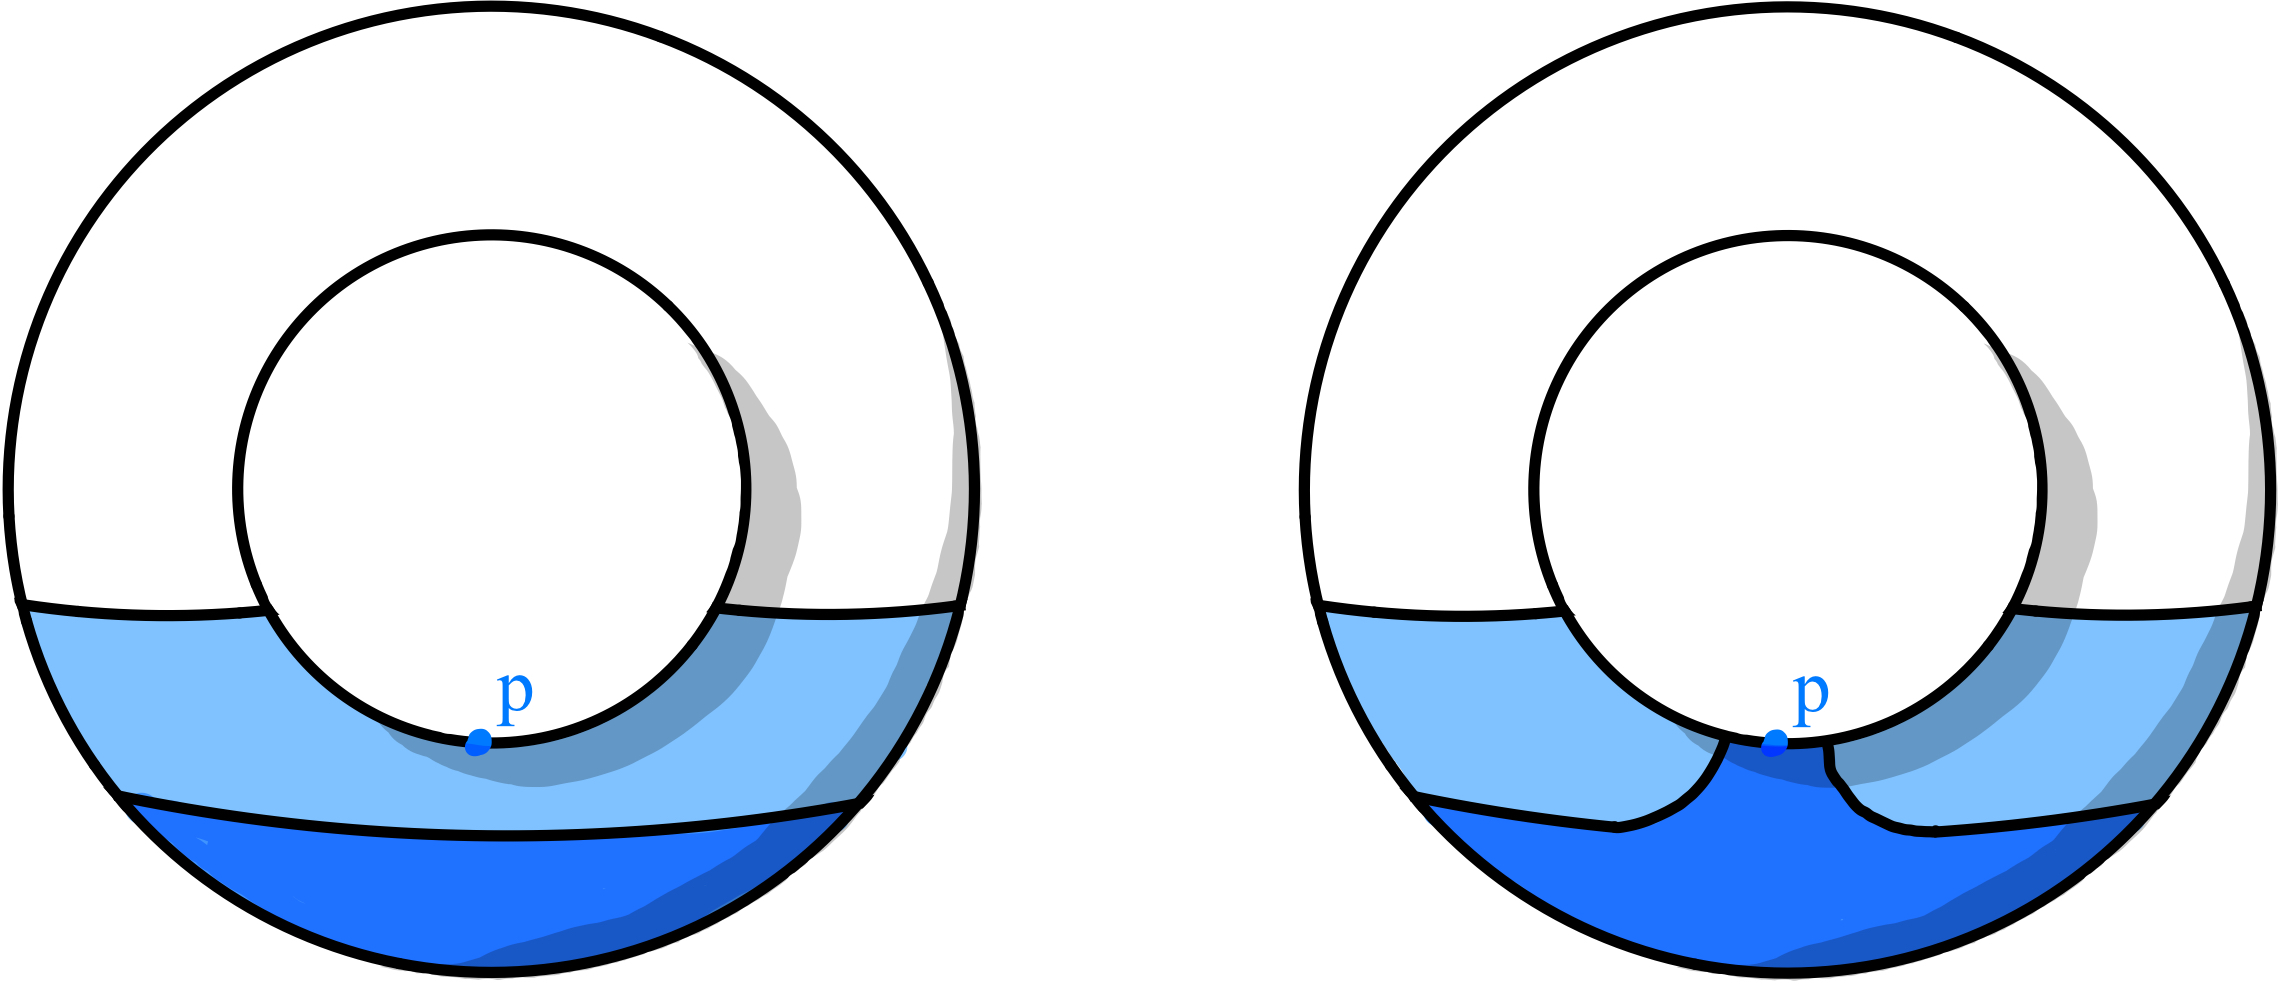
\includegraphics[width=0.8\linewidth]{../resources/Me-Diagram5-sublevelsets-of-f-and-F.jpeg}
        \label{fig:me-diagram5}
        \caption{Die Niveaumengen von $f$ (links) und $F$ (rechts)}
    \end{figure}

    Wir wollen also, dass $M^{c + \varepsilon} = F^{-1}(- \infty, c + \varepsilon]$ 
    gilt und $F^{-1}(-\infty, c - \varepsilon]$ fast dasselbe ist wie 
    $M^{c - \varepsilon}$, nur dass $F^{-1}(-\infty, c - \varepsilon]$ einen "Henkel"
    enthält der den kritischen Punkt $p$ enthält.

    Wir benutzen das Morse-Lemma~\ref{satz: morse-lemma}:
    Wir finden lokale Koordinaten $\phi = (u_1, \dots, u_n)$ in einer Umgebung $U$ von $p$, sodass 
    \[ f = c - u_1 - \dots - u_k + u_{k + 1} + \dots + u_n \]
    und
    \[ u_1 (p) = \dots = u_n(p) = 0 . \]
    Sei $\eps$ ohne Beschränkung der Allgemeinheit klein genug, sodass $f^{-1}[c - \eps, c + \eps]$ 
    kompakt ist und die Kreisscheibe $\{ x \in \R^n : \| x \|^2 \leq 2 \eps \}$ im Bild von $\phi$ 
    enthalten ist. Wähle nun die $k$-Zelle 
    \[ e^k := \{ q \in M : u_1^2 (q) + \dots + u_k^2 (q) \leq \eps \text{ und }
        u_{k + 1} (q) = \dots = u_n (q) = 0 \} . \]
    Wir bekommen folgende Situation:
    \begin{figure}[H]
        \centering
        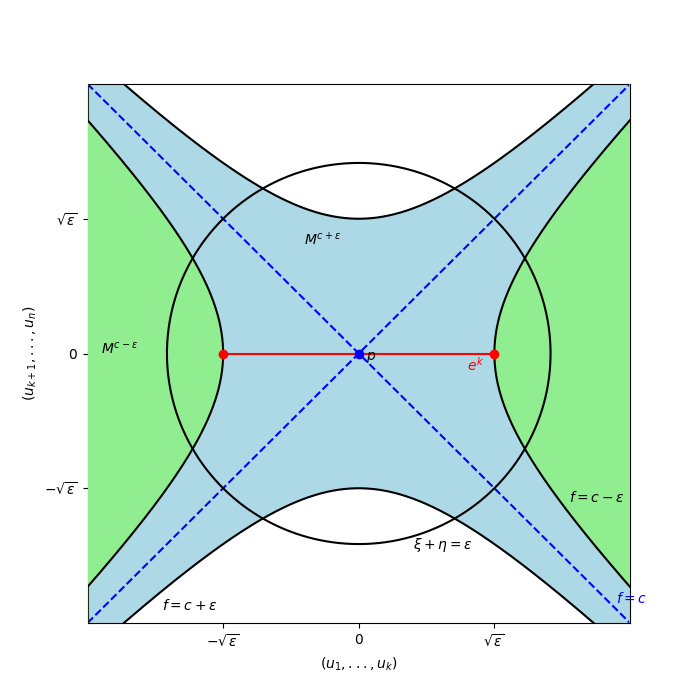
\includegraphics[width=0.45\linewidth]{../resources/Me-Diagram6-U-parameterized.png}
        \label{fig:me-diagram6}
    \end{figure}
    $F$ wird nun so definiert, dass eine Umgebung der $k$-Zelle $e^k$ ein wenig abgesenkt wird.
    Sei $\mu \colon \R \to \R$ eine glatte Funktion mit den Eigenschaften
    \begin{enumerate}
        \item $\mu(0) > \eps$
        \item $\mu (r) = 0$ falls $r \geq 2 \eps$
        \item $-1 < \mu' (r) \leq 0$ für alle $r \in \R$ .
    \end{enumerate}
    Sei dann $F$ außerhalb von $U$ gleich $f$, und innerhalb von $U$ setze
    \[ F = f - \mu ( u_1^2 + \dots + u_k^2 + 2 u_{k + 1}^2 + \dots + 2 u_n^2) . \]
    Man überprüft dann die drei Behauptungen
    \begin{enumerate}
        \item $F^{-1}(- \infty, c + \eps] = M^{c + \eps}$,
        \item $F^{-1}(- \infty, c - \eps]$ ist Deformationsretrakt von $M^{c + \eps}$,
        \item $M^{c - \eps \cup e^k}$ ist Deformationsretrakt von $F^(- \infty, c - \eps]$.
    \end{enumerate}
    Die zweite Behauptung folgt aus dem ersten Deformationslemma.
    
    Den detaillierten Beweis findet man zum Beispiel in \cite{milnor}.
\end{proof}

Mit diesen beiden Aussagen kommt man schon sehr weit. Die berühmten Morse- \\Ungleichungen lassen
sich mit ein bisschen linearer Algebra an exacten Sequenzen leicht daraus folgern. Man kann sogar
zeigen, dass jede Mannigfaltigkeit dein Homotopietypen eines CW-Komplexes 
(siehe Def.~\ref{def: cw-komplex}) besitzt, wie es zum Beispiel Milnor tut. Die Folgenden Kapitel 
geben eine etwas eleganterere Sicht auf die Thematik, die in gewisser Hinsicht stärkere Aussagen
liefert:

\textit{Kompakte} Mannigfaltigkeiten haben nicht nur den selben Homotopie-Typen eines CW-Komplexes, 
sondern sie sind sogar CW-Komplexe, und wir können uns die zelluläre Homologie, die aus der 
CW-Struktur hervorgeht sogar auf eine einfache Art und Weise erklären.

\chapter{Der Morse-Komplex}
In diesem Kapitel wird der Morse Komplex definiert und gezeigt, dass der 
Morse-Komplex ein Kettenkomplex ist.

\section{Die stabile- und instabile Mannigfaltigkeit und die Smale-Bedingung}

\begin{definition}[Stabile- und instabile Mannigfaltigkeit]
    \label{def: stabile und instabile mannigfaltigkeit}
    Es sei $f \colon M \to \R$ eine Morse-Funktion, $p$ ein kritischer Punkt von $f$ und $X$ ein
    Pseudo-Gradientenfeld von $f$. Die stabile Mannigfaltigkeit von $p$ ist die Menge
    \[ \stab (p) = \left\{ q \in M : \lim_{t \to + \infty} \phi_t(q) = p \right\} \]
    und die instabile Mannigfltigkeit ist
    \[ \unst (p) = \left\{ q \in M : \lim_{t \to - \infty} \phi_t(q) = p \right\} . \]
\end{definition}

Bevor wir die stabile- und instabile Mannigfaltigkeit eines kritischen Punktes weiter untersuchen, 
fixieren wir ein Paar Notationen zu Morse Umgebungen. Für das gesamte Kapitel ist diese Vorstellung
von Morse-Umgebungen wichtig.

\begin{definition}[Notationen zu Morse Umgebungen]
    \label{def: notation morse umgebung}
    Zuerst untersuchen wir eine quadratische Formin $\R^n$, die die Form hat wie Funktionen in Morse
    Umgebungen, also $Q \colon \R^n \to \R$ mit
    \[ Q(x_1, \dots, x_n) = - x_1^2 - \dots - x_k^2 + x_{k + 1}^2 + \dots + x_n^2 \]
    für ein $1 \leq k \leq n$.
    Mit $x_- := (x_1, \dots x_k)$ und $x_+ := (x_{k + 1} \dots x_n)$ gilt dann
    \[ Q = - \| x_- \|^2 + \| x_+ \|^2 . \]
    Der Gradient von $Q$ ist mit dem Standardskalarprodukt auf $\R^n$
    \[ \grad Q (x_-, x_+) = 2(x_-, x_+) . \]
    Es seien $\eps, \eta > 0$. Dann definiere die Menge
    \[ U(\eps, \eta) := \left\{ x \in \R^n : - \eps \leq Q(x) \leq \eps 
    \text{ und } \| x_- \|^2 \| x_+ \|^2 \leq \eta(\eps + \eta) \right\} := U . \]
    Wir definieren außerdem
    \begin{align*}
        \del_{\pm} U := & \left\{ x \in U: Q(x) = \pm \eps \text{ und } \|x_{\mp} \|^2 \leq \eta \right\} 
            \text{ und} \\
        \del_0 U := & \left\{ x \in \del U: \| x_- \|^2 \| x_+ \|^2 = \eta(\eps + \eta) \right\} .
    \end{align*}
    Dann setzt sich der Rand von $U$ aus diesen drei Teilen zusammen, also
    \[ \del U = \del_+ \cup \del_- \cup \del_0 . \]
    $\del_0 U$ ist parallel zu den Trajektorien des negativen Gradienten von $Q$. $\del_+ U$ und 
    $\del_- U$ sind orthogonal zu den Trajektorien des negativen Gradienten von $Q$, wobei die 
    Trajektorien in $\del_+ U$ in die Menge $U$ eintreten und sie in $\del_- U$ wieder verlassen. 
    Wir setzen nun $V_- = \langle e_1, \dots, e_k \rangle$ und 
    $V_+ = \langle e_1, \dots, e_n \rangle \subseteq \R^n$. $V_+$ ist der größte Vektorraum, 
    auf dem $\opd^2 Q (0) (\cdot, \cdot)$ positiv definit ist und $V_-$ der größte Vektorraum, auf dem 
    $\opd^2 Q (0) (\cdot, \cdot) (0)$ negativ definit ist. 
    Es gilt 
    \[ \del U \cap V_{\pm} \subseteq \del_{\pm} U . \]
    $0$ ist der einzige kritische Punkt von $Q$ und ist offensichtlich nicht degeneriert. Damit ist $Q$
    eine Morse Funktion und es gilt 
    $\stab (0) = V_+$ und $\unst (0) = V_-$.

    Ist nun $f \colon M \to \R$ eine Morse Funktion, $p$ ein kritischer Punkt von $f$ und $(V, \psi)$
    eine Morse Umgebung von $p$, dann gilt $f \circ \psi^{-1} = Q + f(p)$. Sind $\eps$ und $\eta$
    klein genug, dann ist $U \subset \psi(V)$. Wir nennen 
    $\Omega (p, \eps, \eta) = \Omega (p) = \psi^{-1}(U)$, und 
    $\del_{\pm} \Omega (p) = \psi^{-1}(\del_{\pm}U)$ und $\del_0 \Omega (p) = \psi^{-1} (\del_0 U)$.
    Dann ist 
    \[ \psi(\stab (p) \cap \Omega (p)) = V^+ \cap U \] 
    und 
    \[ \psi(\unst (p) \cap \Omega (p)) = V^- \cap U . \]
    Wir können uns also mit dieser Notation die stabile- und instabile Mannigfaltigkeit (wenigstens 
    in einer Umgebung von $p$) sehr gut vorstellen.

    \begin{figure}[ht]
        \centering
        \begin{minipage}{.4\textwidth}
          \centering
          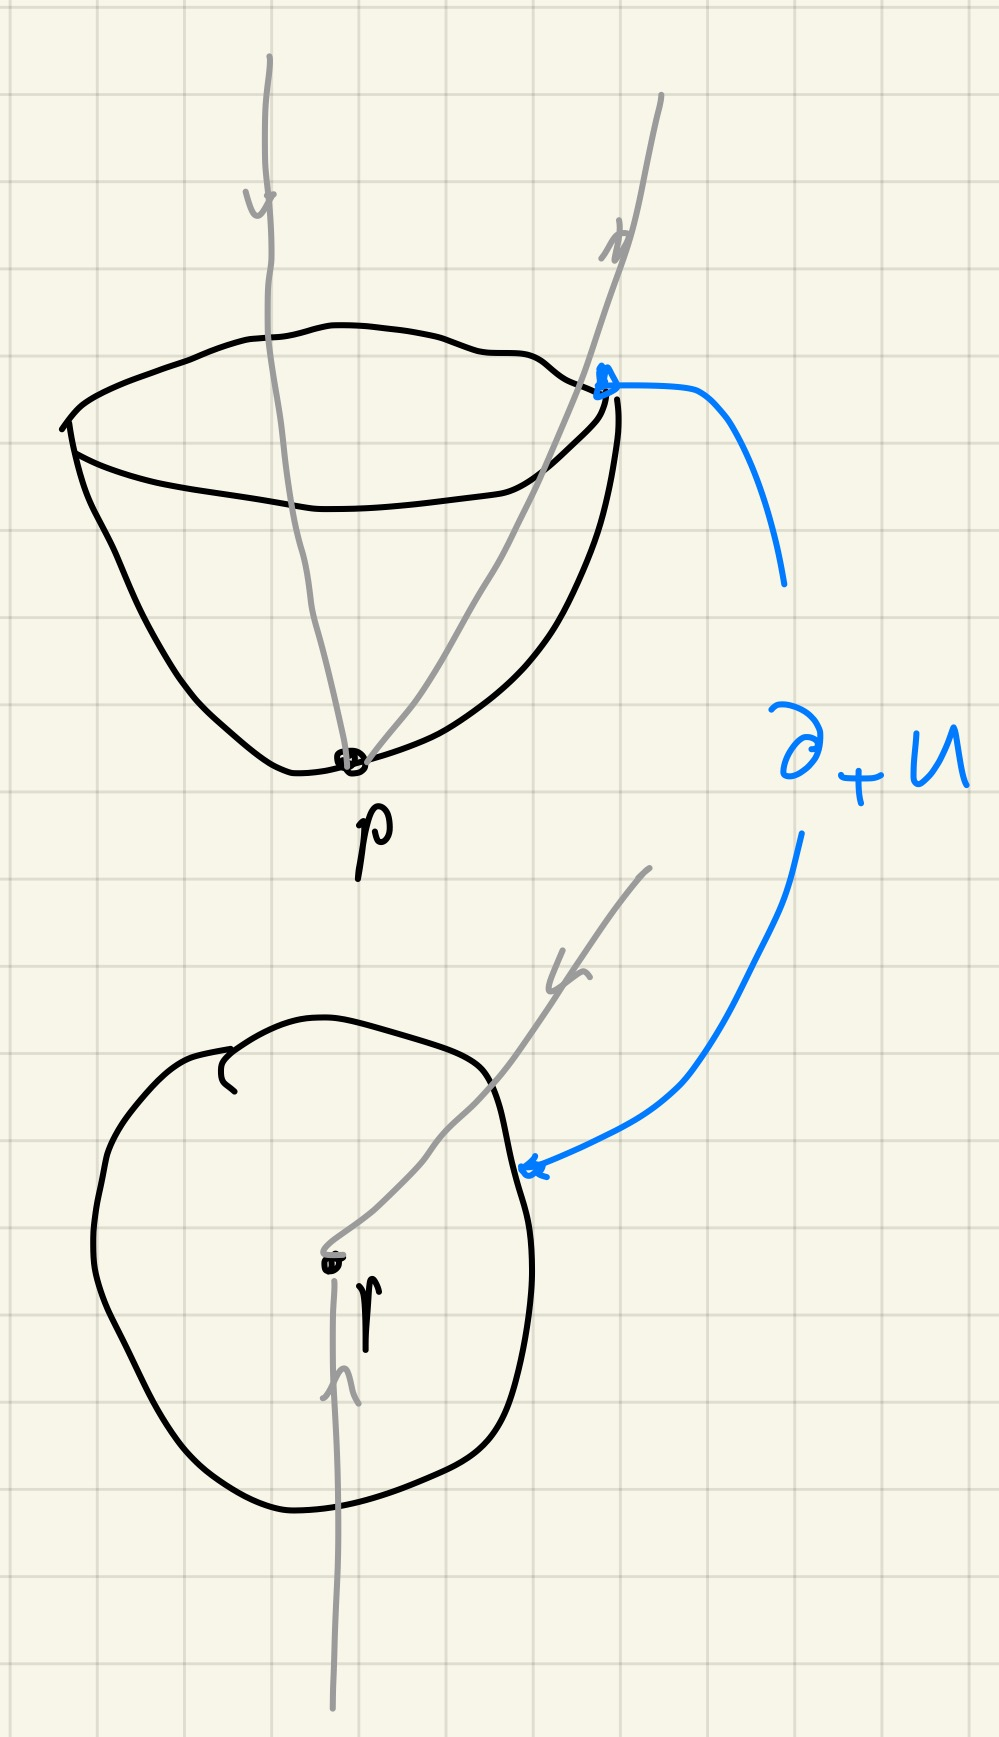
\includegraphics[width=.4\linewidth]{../resources/def-notation-morse-umgebung-1.JPG}
          \captionof{figure}{Index $0$}
          \label{fig: morse umgebung ind 0}
        \end{minipage}%
        \begin{minipage}{.4\textwidth}
          \centering
          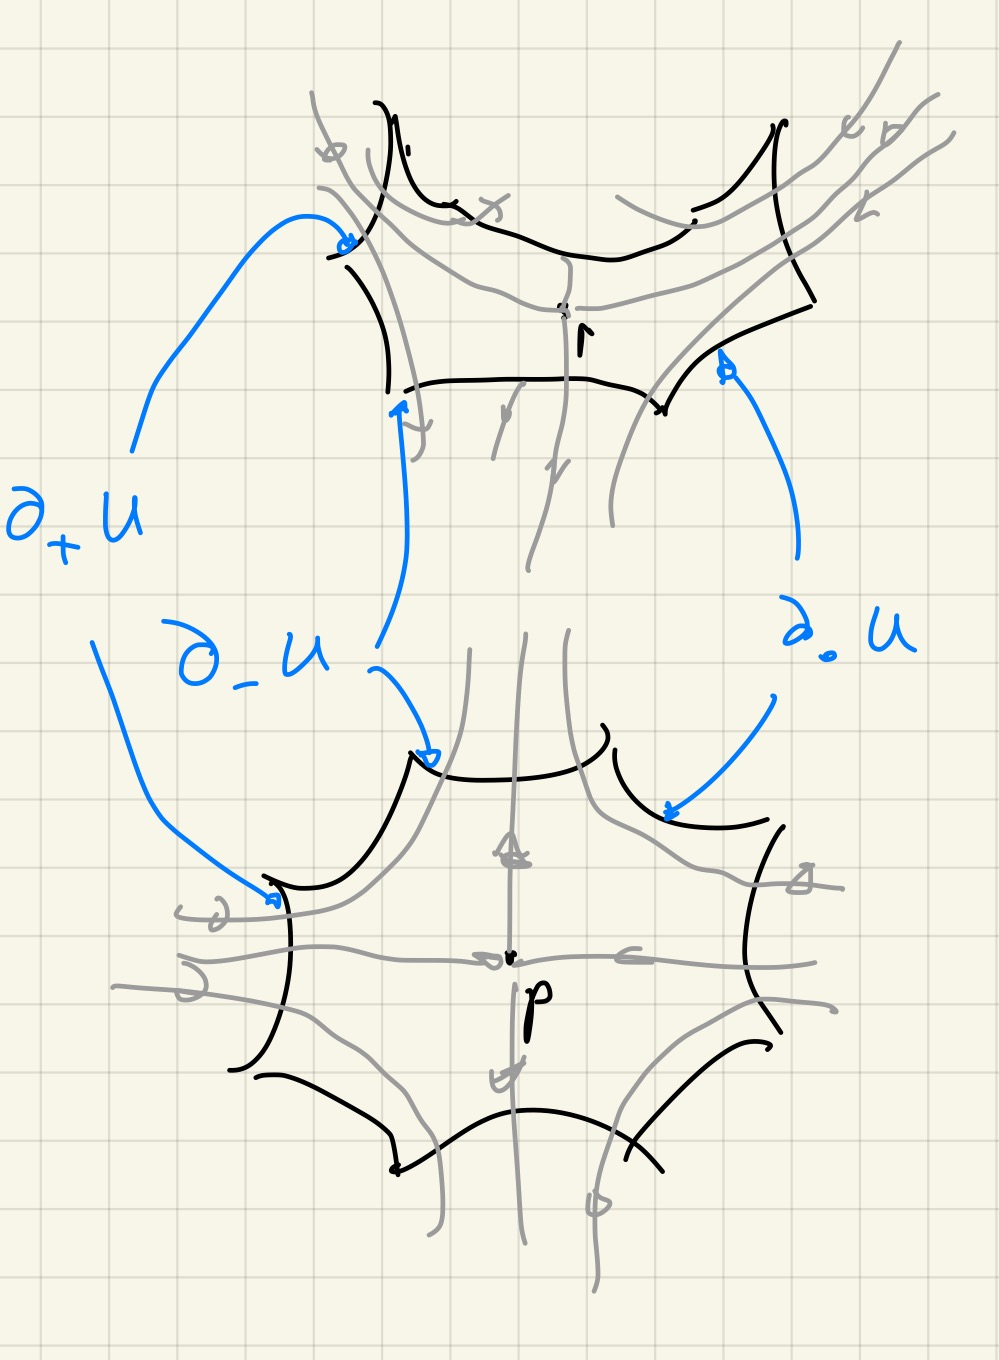
\includegraphics[width=.4\linewidth]{../resources/def-notation-morse-umgebung-2.JPG}
          \captionof{figure}{Index $k$, $0 < k < n$}
          \label{fig: morse umgebung ind k}
        \end{minipage}
    \end{figure}

    $\eps$ und $\eta$ werden häufig in der Notation ausgelassen.
\end{definition}

Mit dieser Vorstellungen von Morse-Funktinoen können wir die folgende Aussage beweisen.

\begin{prop}
    Ist $f \colon M \to \R$ eine Morse Funktion und $p$ ein kritischer Punkt von $f$, dann sind
    $\stab (p)$ und $\unst (p)$ Mannigfaltigkeiten mit 
    \[ \dim \unst (p) = n - \dim \stab (p) = \Index (p) \]
\end{prop}

\begin{proof}
    Es sei $(\psi, V)$ eine Morse Karte um $p$ und $\Omega(p) \subseteq V$ in einer Form wie 
    in ~\ref{def: notation morse umgebung}. Es sei außerdem $\phi$ der Fluss eines 
    Pseudo-Gradientenfeldes von $f$. Dann ist 
    \[ \Phi \colon \del_+ \Omega (p) \cap \stab (p) \times \R \to M ; \; \Phi (q, t) = \phi_t(q) \]
    eine Einbettung und es gilt 
    \[ \stab (p) = \Ima \Phi \cup \psi^{-1}(U \cap V_+) . \]
    Tatsächlich ist 
    \[ \stab (p) - \Ima \Phi = \{ p \} , \]
    denn $\lim_{t \to \infty} \phi_t(q) = p$ für $q \in \del_+ \Omega (p) \cap \stab (p)$. 
    Außerdem ist 
    \[ \del_+ U \cap V_+ = \{ x \in \R^n: \| x_+ \|^2 = \eps \} \diffeo S^{n - k - 1} , \] 
    denn für alle $x \in V_+$ gilt sowieso schon $x_- = 0$. Also ist $\stab(p)$ diffeomorph zum Raum 
    $S^{n - k - 1} \times (-\infty, \infty]/\sim$, in dem alle Punkte in $\infty$ zusammengeklebt 
    werden. Dieser Quotient ist wiederum diffeomorph zur offenen Kreisscheibe mit Dimension $n - k$.
    Genauso zeigt man, dass $\unst (p)$ diffeomorph zur offenen Kreisscheibe mit Dimension $k$ ist.
\end{proof}

\begin{prop}
    \label{prop: trajektorien enden in kritischen punkten}
    Es sei $f \colon M \to \R$ eine Morse-Funktion und $X$ ein Pseudo-\\Gradientenfeld von $f$. 
    Sei außerdem $M$ kompakt. Ist dann $\phi$ der Fluss von $X$, dann existieren für jeden Punkt 
    $p \in M$ kritische Punkte $q$ und $r$ von $f$, sodass
    \[ \lim_{t \to + \infty} \phi_t(p) = q \;\;\; 
    \text{ und } \;\;\; \lim_{t \to -\infty} \phi_t(p) = r \]
\end{prop}

\begin{proof}
    Wir zeigen die erste Aussage. Seien für jeden kritischen Punkt $p$ $(U_p, \psi_p)$ Morse Karten.
    Es ist $\lim_{t \to + \infty} \phi_t(q) = p$, genau dann wenn
    der Fluss $\phi_{\bullet}(q)$ den Punkt $q$ irgendwann in die Umgebung 
    $\del_+ \Omega (p) \cap \stab(p)$ transportiert. Angenommen $\phi_{\bullet}(q)$ transportiert
    $q$ nie zu einem kritischen Punkt. Jedes mal wenn $\phi_{\bullet}(q)$ also ins Innere einer
    Morse-Umgebung $U_q$ gerät, muss diese Umgebung auch wieder verlassen werden. Da 
    $f \circ \phi_{bullet}(q)$ monoton ist, kann nachdem $\phi_{bullet}(q)$ die Morse-Umgebung 
    $\Omega (p)$ verlassen hat, nie wieder zu dieser zurückgekehrt werden.
    Sei also 
    \[ \Omega = \bigcup_{p \in \Crit(f)} \Omega (p) \]
    und $t_0$ der Zeitpunkt an dem $\phi_{\bullet} (q)$ die Umgebung $\Omega$ das letzte mal verlässt.
    Da $M - \Omega$ keine kritischen Punkte von $f$ enthält existiert ein $\eps_0 > 0$, sodass für 
    alle $x \in M - U$ gilt 
    \[ \opd f (x) ((X(x))) \leq - \eps_ . \]
    Wir rechnen also: Für jedes $t \geq t_0$ gilt
    \begin{align*}
        f(\varphi_t(q) - f(\varphi_{t_0}(q))) = & 
            \int_{t_0}^t \derive[f \circ \phi_{\bullet}(q)]{s} (s) \opd s \\
        = & \int_{t_0}^t \opd f (\phi_s(q)) (X(\phi_s(q))) \opd s \\
        \leq & - \eps_0 (t - t_0) . 
    \end{align*}
    Also für $t \to + \infty$ gilt $f(\phi_t(p)) \to - \infty$. Das kann aber nicht sein, denn da 
    $M$ kompakt ist und $\R$ Hausdorff, ist $f$ eigentlich, also ist $\Ima f$ kompakt. 
    \todo{stimmt das?} Also kann $\phi_{\bullet}(p)$ 
    nicht alle $U_q$ verlassen. aber dann ist 
    \[ \lim_{t \to + \infty} \phi_t(q) = p \]
    für einen kritischen Punkt $p$.
    Genauso zeigt man, dass $\lim_{t \to - \infty} \phi_t(p) = r$ für einen kritischen Punkt $r$.
\end{proof}

\begin{definition}[Smale-Bedingung]
    \label{def: smale-bedingung}
    Es sei $M$ eine Mannigfaltigkeit und $U$ und $V$ Untermannigfaltigkeiten von $M$. Wir sagen 
    $U$ und $V$ sind \textit{transversal} und schreiben $U \pitchfork V$, falls für alle Punkte 
    $p \in U \cap V$ gilt 
    \[ T_pU + T_pV = T_pM . \]
    Ein Vektorfeld $X \in \VFs (M)$ heißt \textit{transversal} zur Untermannigfaltigkeit $U$, falls 
    für alle $p$ in $U$ gilt 
    \[ \langle X(p) \rangle + T_pU = T_pM . \]

    Sei nun $f \colon M \to \R$ eine Morse Funktion und $X$ ein Pseudo-Gradientenfeld von $f$. Dann sagen
    wir, dass $X$ die \textit{Smale-Bedingung} erfüllt, falls für alle kritischen Punkte $p$ und $q$ von 
    $f$ gilt 
    \[ \stab (p) \pitchfork \unst (q) . \]
    Ein Paar $(f, X)$ aus einer Morse-Funktion $f$ und einem Pseudo-Gradientenfeld $X$, das die 
    Smale-Bedingung erfüllt, nennt man \textit{Morse-Smale Paar}.
\end{definition}

\begin{prop}
    \label{prop: schnitt von transversalen untermannigfaltigkeiten}
    Sind $U_1$ und $U_2$ Untermannigfaltigkeiten von einer $n$-\\
    dimensionalen Mannigfaltigkeit $M$ mit 
    Dimensionen $d_1$ und $d_2$, sodass 
    \[ U_1 \pitchfork U_2 , \]
    dann ist $U_1 \cap U_2$ eine Untermannigfaltigkeit von $M$ mit Dimension $d_1 + d_2 - n$.
\end{prop}

\begin{proof}
    Es sei $p \in U_1 \cap U_2$. Da $U_1$ und $U_2$ Untermannigfaltigkeiten sind existieren 
    Karten $(\phi_1, V_1)$ und $(\phi_2, V_2)$ von $M$, sodass 
    \[ \phi_1 = (\phi_1', \phi_1'') \colon V_1 \to 
        \Omega_1 \times \Omega_1' \subseteq \R^{d_1} \times \R^{n - d_1} \]
    mit $\phi_1(V_1 \cap U_1) = \Omega_1 \times \{ 0 \}$ und 
    \[ \phi_2 = (\phi_2', \phi_2'')\colon V_2 \to 
        \Omega_2 \times \Omega_2' \subseteq \R^{d_2} \times \R^{n - d_2} \]
    mit $\phi_2(V_2 \cap U_2) = \Omega_2 \times \{ 0 \}$. Definiere 
    \[ \phi'' = (\phi_1'', \phi_2'') \colon 
        M \supseteq V_1 \cap V_2 \to \R^{n - d_1} \times \R^{n - d_2}. \]
    Dann ist 
    $(\phi'')^{-1}(0) = (U_1 \cap V_1) \cap (U_2 \cap V_2) = (U_1 \cap U_2) \cap (V_1 \cap V_2) := V$.
    Wir wollen nun den Satz über reguläre Werte anwenden, aber dafür müssen wir zeigen, dass 
    $\opd \phi'' (p)$ surjektiv ist. Bemerke, dass 
    $\opd \phi'' (p) = \opd (\phi''_1, \phi''_2) (p) = (\opd \phi''_1 (p), \opd \phi''_2 (p))$.
    Es sei $v \in T_p \R^{n - d_1}$ und $w \in T_p\R^{n - d_2}$. Da $\opd \phi''_1 (p)$ und 
    $\opd \phi''_2 (p)$ surjektiv sind, und da $U_1$ und $U_2$ transversal sind, 
    existieren $v_1' + v_2', w_1' + w_2' \in T_pU_1 + T_pU_2$, sodass 
    $\opd \phi''_1 (p) (v_1 + v_2) = \opd \phi''_1 (p) (v_2) = v$ und 
    $\opd \phi''_2 (p) (w_1 + w_2) = \opd \phi''_2 (p) (w_1) = w$.
    Die ersten Gleichheiten gelten, da $T_p U_1$ der Kern von $\opd \phi''_1 (p)$ und 
    $T_p U_2$ der Kern von $\opd \phi''_2 (p)$ sind. Dann gilt
    \[ \opd \phi'' (p) (w_1' + v_2')  = 
        ( \opd \phi''_1 (p) (v_2'), \opd \phi''_2 (p) (w_1')) = (v, w) . \]
    Wir können also den Satz über reguläre Werte anwenden, dann ist $V$ eine Untermannigfaltigkeit
    mit Dimension $n - ((n - d_1) + (n - d_2)) = d_1 + d_2 - n$. Dann ist auch $U_1 \cap U_2$
    eine Untermannigfaltigkeit von Dimension $d_1 + d_2 - n$.
\end{proof}

Dann folgt direkt:

\begin{prop}
    Es sei $f \colon M \to \R$ eine Morse Funktion und $p$ und $q$ kritische Punkte von mit Index $k_1$
    und $k_2$ respektive. Falls $X$ die Smale-Bedingung erfüllt ist
    \[ \mathcal{M} (p, q) := \unst (p) \cap \stab (q) = 
        \left\{ r \in M : \lim_{t \to - \infty} \phi_t(p) \text{ und } 
        \lim_{t \to + \infty} \phi_t(q) \right\} \]
    ist eine Mannigfaltigkeit mit Dimension $k_1 - k_2$.
\end{prop}

Der Raum $\mathcal{M} (p, q)$ beinhaltet alle Punkte, die auf Trajektorien zwischen den kritischen
Punkten $p$ und $q$ liegen. 

\todo{Zeichnung}

\begin{prop}
    \label{prop: wohldefiniertheit von Lt}
    $\R$ wirkt via $(p, t) \mapsto \phi_t(p)$ auf $\mathcal{M}(p, q)$. Sind $p$ und $q$ kritische 
    Punkte mit $p \neq q$ und Indizes $k_1$ und $k_2$, dann ist 
    \[ \Lt (p, q) = \mathcal{M} (p, q) / \R \]
    eine $k_1 - k_2 - 1$-dimensionale Mannigfaltigkeit und es gilt 
    \[ \Lt (p, q) \diffeo \mathcal{M} (p, q) \cap f^{-1}(c) \]
    für einen regulären Wert $c$ zwischen $f(p)$ und f(q)
    (Wir können ohne Beschränkung der Allgemeinheit annehmen, dass $f(p) \neq f(q)$).
\end{prop}

\begin{proof}
    Die Gruppenwirkung ist frei, denn in $\mathcal{M} (p, q)$
    sind keine kritischen Punkte, da $p \neq q$. Es sei $x$ in $\mathcal{M} (p, q)$. 
    Ist nun $t \neq 0$, dann gilt da $f \circ \phi_{\bullet}(x)$ streng monoton ist 
    $f(\phi_t(x)) \neq f(\phi_0(x)) = f(x)$, also $\phi_t(x) \neq x$.

    Es sei nun $c$ ein regulärer Wert zwischen $f(p)$ und $f(q)$. $f^{-1}(c)$ ist eine 
    $n - 1$-dimensionale Mannigfaltigkeit, und für das Pseudo-Gradientenfeld $X$ gilt 
    $X \pitchfork f^{-1}(c)$, und da für jeden Punkt $a$ gilt $X(a) \in T_a \mathcal{M} (p, q)$
    ist $f^{-1}(c) \cap \mathcal{M} (p, q)$ eine $k_1 - k_2 - 1$-dimensionale Mannigfaltigkeit.
    Sei 
    \[ \iota \colon \mathcal{M} (p, q) \cap f^{-1}(c) \to \mathcal{M}(p, q)\] 
    die Inklusion und 
    \[ p \colon \mathcal{M} (p, q) \to \Lt (p, q) \] 
    die Quotientenabbildung. $p \circ \iota$ ist bijektiv und stetig, und ist 
    $U \subseteq \mathcal{M} (p, q)$ offen, dann ist $p \circ \iota (U)$ offen in $\Lb (p, q)$. 
    Also ist $p \circ \iota$ ein Homeomorphismus und $\Lt (p, q)$ ist Hausdorff, also ist $\Lt (p, q)$
    eine Mannigfaltigkeit, und es gilt sogar
    \[ \Lt (p, q) \diffeo \mathcal{M} (p, q) \cap f^{-1}(c) \]
\end{proof}

Der Raum $\Lt (p, q)$ enthält für jede Trajektorie, die zwischen den kritischen Punkten $p$ und $q$ 
verläuft einen Repräsentanten. Später wird $\Lt (p, q)$ benutzt, um den Morse-Komplex zu definieren.
Die Smale Bedingung ist also für unsere Zwecke wichtig.

Wir gewinnen auch eine wichtige Erkenntnis: 

\begin{corollary}
    Der Index von kritischen Punkten verringert sich entlang von Trajektorien. Denn falls 
    $\Index (p) \leq \Index (q)$, dann ist die Dimension von $\Lt (p, q)$
    kleiner $0$, also ist dann $\Lt (p, q) = \varnothing$.
\end{corollary}

Um den Morse Komplex für jede (kompakte) Mannigfaltigkeit definieren zu können, muss noch gezeigt
werden, dass auf jeder Mannigfaltigkeit tatsächlich ein Morse-Smale Paar existiert. 
Sogar noch stärker ist die folgende Aussage:

\begin{theorem}[Satz von Smale-Kupta]
    Es sei $M$ eine Mannigfaltigkeit mit Rand und $f$ eine Morse-Funktion. Es sei $\Omega$ die 
    Vereinigung von Morse-Umgebungen von allen kritischen Punkten. Sei $X$ ein Pseudo-Gradientenfeld 
    von $f$. Dann existiert ein Pseudo-Gradientenfeld $X'$ von $f$, das die Smale Bedingung erfüllt, 
    das innerhalb von $\Omega$ gleich $X$ ist und für das gilt:

    Für jedes $\eps > 0$, jeden Atlas $(\phi_i, U_i)_{i \in I}$ von $M$ und alle $i \in I$ existiert 
    für jede Kompakte Teilmenge $K_i \subseteq U_i$ ein Vektorfeld $X'$, sodass 
    \[ \| \opd \phi_i^{-1} (\cdot) (X') - \opd \phi_i^{-1} (\cdot) (X) \| < \eps . \]
\end{theorem}

\begin{proof}
    Der Satz wurde von S. Smale in \cite{smale1} bewiesen.
\end{proof}
\section{Der Morse-Komplex und der Raum der gebrochenen Trajektorien}

Wir sind nun bereit, den Morse-Komplex mit Koeffizienten in $\F_2$ (wenigstens) hinzuschreiben.
Wir fixieren für den gesamten Abschnitt eine glatte \textbf{kompakte} Mannigfaltigkeit $M$ und ein
Morse-Smale Paar $(f, X)$. Die Notation, die wir zu Morse-Umgebungen 
in~\ref{def: notation morse umgebung} entwickelt haben wird weiterhin wichtig sein. 
Dann definiere $C_k (M, (f, X))$ als das $\F_2$-Modul, 
das von den kritischen Punkten von $f$ mit Index $k$ erzeugt wird, also
\[ C_k = \left\{ \sum_{p \, \in \, \Crit_k (f)} a_p \cdot p : a_p \in \F_2 \right\} . \] 
Außerdem sei 
$n_X(p, q) = \# \Lt (p, q) \mod 2$. Dann definiere für einen kritischen Punkt $p$ mit Index $k + 1$:
\[ \del_X (p) := \sum_{q \, \in \, \Crit_{k}(f)} n_X(p, q)p . \]

Das Ziel dieses Abschnittes ist es zu zeigen, dass der Komplex $C_{\ast}(M, (f, X))$ wohldefiniert
ist, also dass gilt $n_X (p, q) < \infty$, und dass es ein Kettenkomple ist, also dass 
$\del_X \circ \del_X = 0$. Sobald das gezeigt wurde ist es recht leicht, den Komplex auch über die 
ganzen Zahlen zu definieren.

\subsection*{Wohldefiniertheit}

\begin{definition}[Der Raum der gebrochenen Trajektorien]
    \label{def: raum der gebrochenen trajektorien}
    Es seien $p$ und $q$ kritische Punkte von $f$. Der \textit{Raum der gebrochenen Trajektorien} ist
    \[ \Lb (p, q) = 
        \bigcup_{k \in \N} \left( \bigcup_{\substack{c_1, \dots, c_{k - 1} \\ \in \Crit(f)}} 
            \Lt (p, c_1) \times \Lt (c_1, c_2) \times \dots 
                \times \Lt (c_{k - 2}, c_{k - 1}) \times \Lt (c_{k - 1}, q) \right) . \]
\end{definition}

Obwohl die Formulierung recht sperrig wirkt ist sie doch intuitiv: 
$\ell \in \Lt (p, q)$ ist eine \glqq Verbindung\grqq{} zwischen den kritischen Punkten $p$ und $q$ 
entlang des Pseudo-Gradientenfeldes $X$. Ein Element 
$(\ell_1, ..., \ell_k) \in \Lt (p, c_1) \times \dots \times \Lt (c_{k - 1}, q) \subseteq \Lb (p, q)$
ist eine \glqq Verbindung\grqq{} zwischen $p$ und $q$ entlang des Pseudo-Gradientenfeldes $X$, die noch 
bei den kritischen Punkten $c_1, \dots, c_{k - 1}$ \glqq Halt\grqq{} macht. 

\todo{Zerichnung: gebrochene Trajektorien}

Offensichtlich gilt:
\begin{itemize}
    \item Für jedes $\ell \in \Lt (p, c_1) \times \dots \times \Lt (c_{k - 1}, q)$ gilt 
        $\Index (p) < \Index (c_1) < \dots < \Index (c_{k - 1}) < \Index (q)$, denn falls dies nicht
        der Fall ist, ist mindestens einer der Faktoren leer. 
    \item Ist $\Index (p) = \Index (q) + 1$, so ist $\Lb (p, q) = \Lt (p, q)$.
    \item Ist $\Index (p) = \Index (q) + 2$, so ist 
        $\Lb (p, q) = \Lt (p, q) \cup \bigcup_{c \in \Crit (f)} \Lt(p, c) \times \Lt(c, q)$
\end{itemize}
Tatsächlich sind die beiden letzten Fälle die, die wir am meisten untersuchen werden.
Wir werden sehen, dass man, wie mit der Notation angedeutet, $\Lb (p, q)$ mit einer Topologie 
ausstatten kann, sodass es die Kompaktifizierung von $\Lt (p, q)$ ist. (In der Tat ist ja 
$\Lt (p, q) \subseteq \Lb (p, q)$).

\begin{definition}[Topologie von $\Lb (p, q)$]
    Ese seien $p$ und $q$ kritische Punkte von $f$. Wir erinnern uns an unsere Vorstellung von Morse-
    Umgebungen $\Omega(p)$ wie in~\ref{def: notation morse umgebung}.
    Es sei
    \[ \ell = (\lambda_1, \dots, \lambda_k) 
        \in \Lt (p, c_1) \times \dots \times \Lt(c_{k - 1}, q) \subseteq \Lb (p, q) . \]
    Seien $U_i = \Omega(c_i)$ Morse Umgebungen von $c_i$ und $U_0$ und $U_k$ Morse 
    Umgebungen von $p$ und $q$. $\lambda_i \cap \del_+ U_i$ ist der Punkt, an dem $\lambda_i$
    in $U_i$ eintritt, und $\lambda_{i + 1} \cap \del_- U_i$ ist der Punkt, an dem 
    $\lambda_{i + 1}$ die Umgebung $U_i$ verlässt. Es sei $U_i^-$ eine Umgebung von 
    $\lambda_i \cap \del_+ U_i$ in 
    $\del_+ U$ und $U_i^-$ eine Umgebung von $\lambda_{i + 1} \cap \del_- U_i$ in $\del_- U_i$. 
    Seien dann $U^- = \bigcup U_i^-$ und $U^+ = \bigcup U_i^+$. Dann definiere die Menge 
    $\mathcal{U} (\ell, U^-, U^+)$ wie folgt:

    Wir sagen 
    $\ell' = (\mu_1, ..., \mu_{k'}) \in \Lt (p, c_{i_1}) \times \dots \times \Lt (c_{i_{k'-1}}, q)$
    ist in $\mathcal{U}(\ell, U^-, U^+)$ enthalten, falls $\mu_j \cap U_j^+ \neq \varnothing$
    und $\mu_j \cap U_{j + 1}^- \neq \varnothing$. 

    Eine Menge $\mathcal{W} \subseteq \Lb (p, q)$ heißt dann \textit{offen}, falls für alle 
    $\ell \in V$ Umgebungen $U_{\ell}^+$ und $U_{\ell}^-$ wie oben existieren, sodass 
    \[ \mathcal{U}(\ell, U_{\ell}^+, U_{\ell}^-) \subseteq V . \]
\end{definition}

\begin{remark}
    Die Topologie von $\Lt(p, q)$ als Quotient stimmt mit der von $\Lb(p, q)$ überein.
    Dies ist wieder ersichtlich, wenn wir uns $\Lt (p, q)$ als Schnitt 
    $\mathcal{M} (p, q) \cap f^{-1}(c)$ vorstellen; Die $U^-$ beziehungsweise $U^+$ sind nur 
    offene Umgebungen in den Niveaumengen.
\end{remark}

\begin{prop}
    \label{prop: Lb ist kompakt}
    Es seien $p$ und $q$ kritische Punkte von $f$. Dann ist $\Lb (p, q)$ kompakt.
\end{prop}

Um diese Proposition zu beweisen benötigen wir noch ein Lemma:

\begin{lemma}
    \label{lemma: konvergenz einer folge}
    Es sei $x \in M$ \emph{kein} kritischer Punkt von $f$. Sei außerdem $(x_n)_n$ eine Folge in
    $M$ die gegen $x$ kovnvergiert und seien $y_n$ und $y$ Punkte, die auf den selben Trajektorien
    wie $x_n$ und $x$ liegen. Es gelte außerdem $f(y_n) = f(y)$ für alle $n \in \N$. Dann gilt
    \[ \lim_{n \to + \infty} y_n = y . \]
\end{lemma}

\begin{proof}
    Es sei $U$ eine Umgebung von $\Crit (f)$. Dann ist $\opd f (\cdot) (X)$  in $M - U$ nie Null.
    Ähnlich wie im Beweis vom ersten Deformationslemma~\ref{satz: erstes deformationslemma} betrachten 
    wir das Vektorfeld 
    \[ Y = - \frac{1}{\opd f (\cdot) (X)} \cdot X \]
    Auf $M - U$. Sei $\phi$ die von $Y$ erzeugte 1-Parameter Gruppe aus Diffeomorphismen. 
    Da $Y$ in die selbe Richtung zeigt wie $X$, stimmen die Trajektorien von $Y$ mit denen von $X$ 
    überein und außerdem gilt 
    \[ f(\phi_t(z)) = f(z) - t . \]
    Dann gilt
    \begin{align*} 
        \lim_{n \to \infty} y_n  = & \lim_{n \to \infty} \phi_{- f(y_n) + f(x_n)}(x_n) \\
        = & \lim_{n \to \infty} \phi_{- f(y) + f(x_n)}(x_n) \\
        = & \phi_{- f(y) + f(x)}(x) = y
    \end{align*}
\end{proof}

\begin{proof}[Beweis von Proposition~\ref{prop: Lb ist kompakt}]
    Es sei $(\ell_n)_n$ eine Folge in $\Lb (p, q)$. Um zu zeigen, dass $\Lb (p, q)$ kompakt ist
    müssen wir zeigen, dass $(\ell_n)_n$ eine konvergente Teilfolge besitzt.

    Wir nehmen zuerst an, dass für alle $n \in \N$ die Trajektorie $\ell_n \in \Lt (p, q)$.
    Es sei $\ell_n^- \in M$ der Punkt, an dem $\ell_n$ die Morse Umgebung $\Omega(p)$ verlässt 
    und $\ell_n^- \in M$ der Punkt, an dem $\ell_n$ in die Morse Umgebung $\Omega(q)$ eintritt.
    $\ell_n^-$ und $\ell_n^+$ sind im Schnitt von $\del \Omega (p)$ bzw. $\del \Omega (q)$ und 
    der stabilen bzw. instabilen Mannigfaltigkeit. Diese Schnitte sind Kugeloberflächen, also 
    kompakt. Die Folgen $(l_n^-)_n$ und $(\ell_n^+)_n$ haben also konvergente Teilfolgen, wir können 
    demnach ohne Beschränkung der Allgemeinheit annehmen, dass sie konvergent sind. Setze
    \[ \lim_{n \to \infty} \ell_n^- = p^- \text{ und } \lim_{n \to \infty} \ell_n^+ = q^+ . \]
    Sei $\phi$ die von $X$ erzeugte 1-Parameter Gruppe aus Diffeomorphismen, dann ist 
    $\gamma = \phi_{\bullet}(p^-)$ die Trajektorie von $p^-$. Sei 
    $c = \lim_{n \to \infty} \phi_t(p^-)$. Der Punkt $c$ ist nach 
    Proposition~\ref{prop: trajektorien enden in kritischen punkten} ein kritischer Punkt,
    also ist $\gamma \in \Lt (p, c)$.  Es sei $d^+$ der Punkt, an dem $\gamma$ in $\Omega (c)$ 
    eintritt. Da $\phi$ glatt ist, muss für $n$ groß genug auch $\ell_n$ die Morse Umgebung 
    $\Omega (c)$ kreuzen. Sei $d_n^+ \in M$ der Punkt, an dem $\ell_n$ in $\Omega (c)$ eintritt. 
    Dann gilt $d_n^+, d^+ \in \del_+ W$, also gilt $f(d_n^+) = f(d^+)$ für alle $n$. Da $d_n^+$ auf 
    der selben Trajektorie wie $\ell_n^-$ liegt, und $d^+$ auf der selben wie $p^-$,folgt da 
    $\lim \ell_n^- = p^-$ mit dem letzten Lemma~\ref{lemma: konvergenz einer folge}: 
    \[ \lim_{n \to \infty} d_n^+ = d^+ . \]
    Falls $c = q$, dann ist $\lim \ell_n = \gamma \in \Lt (p, q) \subseteq \Lb (p, q)$, also hat 
    dann die Folge $(\ell_n)_n$ eine konvergente Teilfolge. Es sei also $c \neq q$. Dann muss 
    $\ell_n$ die Morse Umgebung $\Omega (c)$ wieder durch einen Punkt $d_n^-$ verlassen. Wie oben 
    können wir ohne Beschränkung der Allgemeinheit annehmen, dass die Folge $(d_n^-)_n$ konvergent 
    ist, da sie zumindest eine konvergente Teilfolge besitzt. Wir definieren dann $d^- := \lim d_n^-$. 
    $d^-$ liegt in der instabielen Mannigfaltigkeit von $c$, denn wäre dies nicht der Fall, dann 
    führt das zu einem Widerspruch:
    
    Angenommen $d^- \notin \unst (c)$. Dann wäre $d^-$ auf der Trajektorie von einem Punkt
    $d^+_{\ast} \in \del_+ \Omega (c)$, der nicht in $\unst (c)$ enthalten ist. Wieder wegen des 
    vorherigen Lemmas~\ref{lemma: konvergenz einer folge} ist dann $\lim d_n^+ = d^+_{\ast}$, also 
    gilt dann $d^+ = d^+_{\ast}$, aber es gilt $d^+ \in \unst (c)$.
    
    Wir können nun wieder mit dem selben Argument zeigen, dass dann die Trajektorie von $d^-$ im
    kritischen Punkt $q$ endet, also liegt dann $\lim \ell_n$ in $\Lt (p, c) \times \Lt (c, q)$.
    \todo{können wir das wirklich?}

    Jetzt fehlt uns noch der allgemeine Fall. Wir müssen also für eine Folge $(\ell_n)_n$ in 
    $\Lb (p, q)$ zeine konvergente Teilfolge finden. Wegen der Glattheit von $\phi$ können wir annehmen,
    dass für $n$ groß genug alle $\ell_n$ die Form 
    \[ \ell_n = (\ell^1_n, \dots, \ell^k_n) \in \Lt (p, c_1) \times \dots \times \Lt (c_{k - 1}, q) \]
    haben. Wir finden mit der vorheringen Überlegung komponentenweise eine Teilfolge, sodass wir 
    für den grenzwert maximal noch $k - 1$ kritische Punkte als \glqq Zwischenstopp\grqq{} einfügen
    müssen. 
\end{proof}

\begin{remark}
    Sind nun $p$ und $q$ kritische Punkte von $f$ mit $\Index (p) = \Index (q) + 1$, dann ist 
    $\Lt(p, q)$ $0$-dimensionale Mannigfaltigkeit. Außerdem ist $\Lt (p, q)$ eine Abgeschlossene
    Teilmenge von $\Lb (p, q)$, und wie wir in der letzten Proposition~\ref{prop: Lb ist kompakt}
    gezeigt haben, ist $\Lb(p, q)$ kompakt, also auch $\Lt(p, q)$, also ist $\Lt (p, q)$ endlich.
    Damit ist schon mal $n_X (p, q)< \infty$, also $C_k(M (f, X))$ wohldefiniert.
\end{remark}

\subsection*{Der Morse Komplex ist ein Kettenkomplex}

Wir wollen zeigen, dass der Morse-Komplex tatsächlich ein Kettenkomplex ist, also dass 
$\del_X \circ \del_X = 0$.
Wir rechnen:
\begin{align*}
    \del_X (\del_X (p)) = & \del_X (\sum_{c \in \Crit_k (f)} n_X (p, c) \cdot c) \\
    = & \sum_{q \in \Crit_{k - 1}(f)} \left( 
        \sum_{c \in \Crit_k (f)} n_X(p, c) \cdot n_X(c, q) \right) \cdot q
\end{align*}
und 
\[ \sum_{c \in \Crit_k (f)} n_X(p, c) \cdot n_X(c, q) = 
\# \left( \bigcup_{c \in \Crit_k (f)} \Lt (p, c) \times \Lt (c, q) \right) \mod 2 . \]
Es genügt also zu zeigen, dass für kritische Punkte $p$ und $q$ mit Index $k + 1$ und $k - 1$
gilt, dass $\# \left( \bigcup_{c \in \Crit_k (f)} \Lt (p, c) \times \Lt (c, q) \right)$ gerade ist.

Wir benutzen die folgende Aussage, ohne sie zu beweisen:

\begin{theorem}[Klassifizierung kompakter 1-Mannigfaltigkeiten]
    \label{satz: klassifizierung kompakter 1-mannigfaltigkeiten}
    Es sei $M$ eine kompakte zusammenhängende Mannigfaltigkeit mit Rand. Dann ist
    \begin{itemize}
        \item $M$ diffeomorph zu $S^1$, falls $\del M = \varnothing$
        \item $M$ diffeomorph zu $[0, 1]$, falls $\del M \neq \varnothing$
    \end{itemize}
\end{theorem}

\begin{proof}
    Ich hab hier die eine gute Quelle gehabt verdammt. \todo{Quelle}
\end{proof}

\begin{theorem}
    \label{satz: gebrochene trajektorien sind 1-dim mannigfaltigkeit}
    Es seien $p$ und $q$ kritische Punkte von $f$ mit $\Index (p) = k + 1$ und $\Index (q) = k - 1$
    für ein $k \in \N_0$. Dann ist $\Lb (p, q)$ eine 1-dimensionale Mannigfaltigkeit mit Rand, und das
    Innere von $\Lb (p, q)$ ist $\Lt (p, q)$.
\end{theorem}

Mit dieser Proposition folgt dann mit der Kalssifizierung von $1$-Mannigfaltigkeiten mit 
Rand~\ref{satz: klassifizierung kompakter 1-mannigfaltigkeiten} schon, dass der Morse Komplex ein
Kettenkomplex ist.

\begin{bigproof}
    Wir wissen schon, dass $\Lt (p, q) \subseteq \Lb(p, q)$ eine $1$-dimensionale Mannigfaltigkeit ist. 
    Um sagen zu können, dass $\Lb (p, q)$ eine $1$-dimensionale Mannigfaltigkeit mit Rand ist, und 
    insbsondere, dass $\Lt (p, q)$ das Innere von $\Lb(p, q)$ ist, reicht die folgende Aussage über 
    $\Lb(p, q)$:
    Es sei $c$ ein weiterer kritischer Punkt mit Index $k$.
    Sei $\lambda_1 \in \Lt (p, c)$ und $\lambda_2 \in \Lt (c, q)$. Dann existiert eine offene Umgebung
    $U \subseteq \Lb (p, q)$ von $(\lambda_1, \lambda_2)$, ein $\delta > 0$ und eine (topologische)
    Einbettung $\psi \colon [0, \delta) \to U$, sodass gelten: 
    \begin{enumerate}
        \item $\psi|_{(0, \delta)}$ ist glatt.
        \item $\psi(0) = (\lambda_1, \lambda_2)$.
        \item $\psi((0, \delta)) \subseteq \Lt (p, q)$.
        \item Für jede Folge $(\ell_n)_n$ in $\Lt (p, q)$ die gegen $(\lambda_1, \lambda_2)$ konvergiert 
            gilt $\ell_n \in \Ima \psi$ für $n$ groß genug.
    \end{enumerate} 
    Die letzte Bedingung stellt sicher, dass sich in $(\lambda_1, \lambda_2)$ keine 
    \say{Kreuzung} befindet (wie zum Beispiel der Klebepunkt bei $S^1 \wedge S^1$).
    Wir begeben uns also auf die (recht lange) Suche nach einer solchen Abbildung $\psi$. 

    Wir machen ein Paar Konstruktionen. Sei $\alpha := f(c)$ und $(V, \kappa)$ eine Morse Karte von
    $c$, $\Omega(c)$ wie in der Notation zu Morse Umgebungen~\ref{def: notation morse umgebung}. 
    Dann sind $f(\del_+ \Omega) = \alpha + \eps$ und $f(\del_- \Omega) = \alpha - \eps$ für ein 
    $\eps > 0$. Außerdem setze
    \begin{align*}
        S_+ (c) := & \stab (c) \cap f^{-1}(\alpha + \eps) \diffeo S^{n - k - 1} \\
        S_- (c) := & \unst (c) \cap f^{-1}(\alpha - \eps) \diffeo S^{k - 1} .
    \end{align*}
    Dass $S_+ (c)$ und $S_- (c)$ diffeomorph zu Sphären sind hatten wir schon vorher gesehen.
    Es sei $a_1 \in M$ der Punkt, an dem $\lambda_1$ auf $\Omega(c)$ trifft, also 
    $a_1 = S_+ (c) \cap \lambda_1$, und $a_2$ der Punkt, an dem $\lambda_2$ die Umgebung $\Omega (c)$ 
    wieder verlässt, also $a_2 = S_- (c) \cap \lambda_2$. $\alpha + \eps$ ist kein kritischer Wert 
    von $f$ und es gilt $f^{-1}(\alpha + \eps) \pitchfork \unst (p)$, also ist mit 
    Proposition~\ref{prop: schnitt von transversalen untermannigfaltigkeiten} 
    $P = f^{-1}(\alpha + \eps) \cap \unst (p)$ eine Mannigfaltigkeit mit Dimension 
    $(n - 1) + (k + 1) - n = k$. Da $X$ die Smale-Eigenschaft erfüllt, $P \subseteq \unst (p)$,
    $S_+ \subseteq \stab(c)$, $P, S_+(c) \subseteq f^{-1}(c + \eps)$ und 
    $\dim P + \dim S_+(c) = n - 1$ gilt $P \pitchfork S_+ (c)$, also ist $P \cap S_+ (c)$
    mit Proposition~\ref{prop: schnitt von transversalen untermannigfaltigkeiten} eine 
    Untermannigfaltigkeit der Dimenion $k + (n - k - 1) - (n - 1) = 0$. Offensichtlich gilt 
    $a_1 \in P \cap S_+ (c)$. Es sei $D^k_{\delta} = \{ x \in \R^k : \| x \| < \delta \}$. Dann 
    existiert eine Umgebung D von $a_1$ in $P$ und ein Diffeomorphismus 
    $\Psi : D \longto D^k_{\delta}$ mit $\Psi(a_1) = 0$, sodass $D \cap S_+ (c) = a_1$ 
    und $D \subseteq \del_+ \Omega (c)$. Wir versuchen die Kernidee des Beweises zu verstehen:

    \begin{figure}
        \centering
        \begin{minipage}{.5\textwidth}
          \centering
          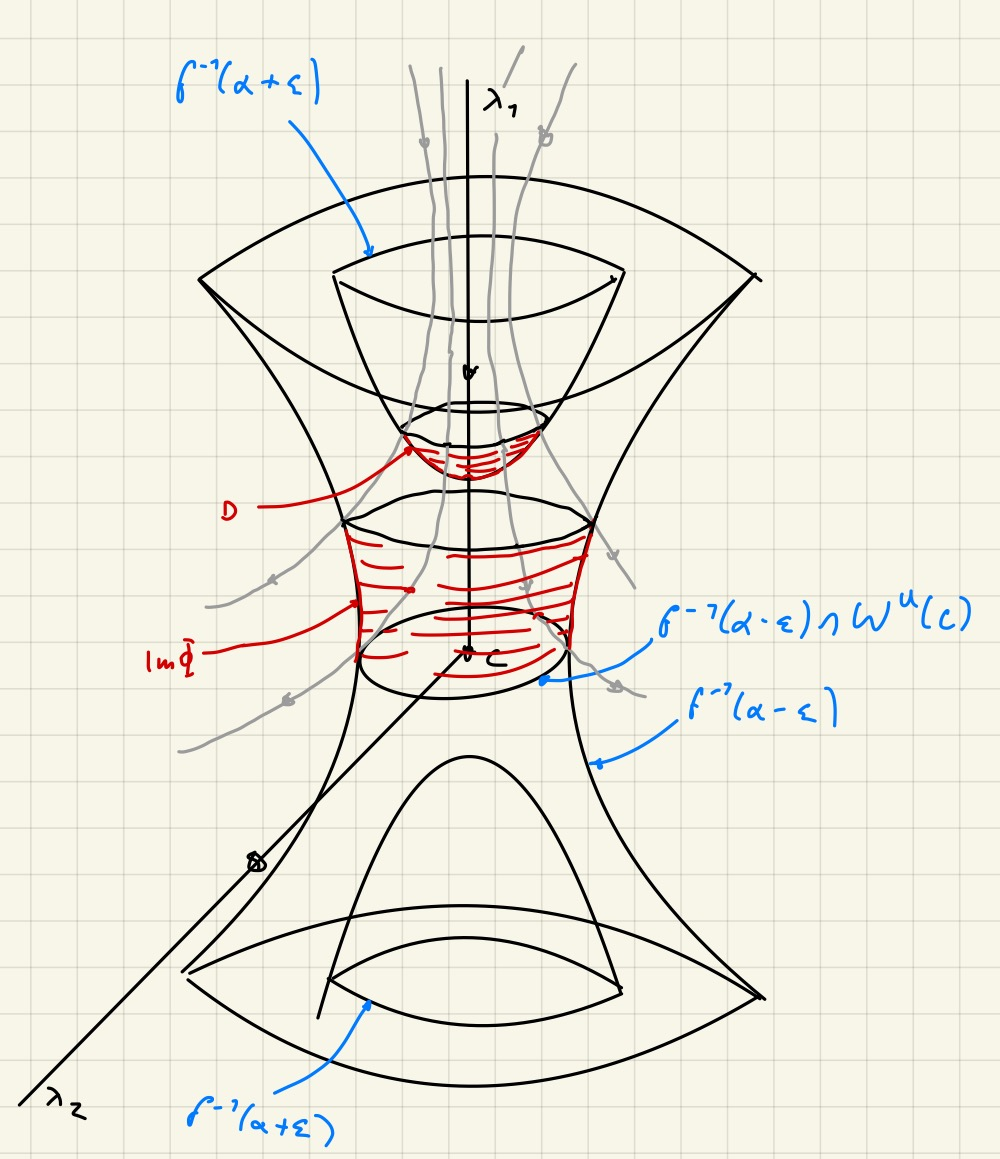
\includegraphics[width=.85\linewidth]{../resources/bew-gebrochene-trajektorien-sind-1-dim-mannigfaltigkeit-1.JPG}
          \captionof{figure}{A figure}
          \label{fig: test1}
        \end{minipage}%
        \begin{minipage}{.5\textwidth}
          \centering
          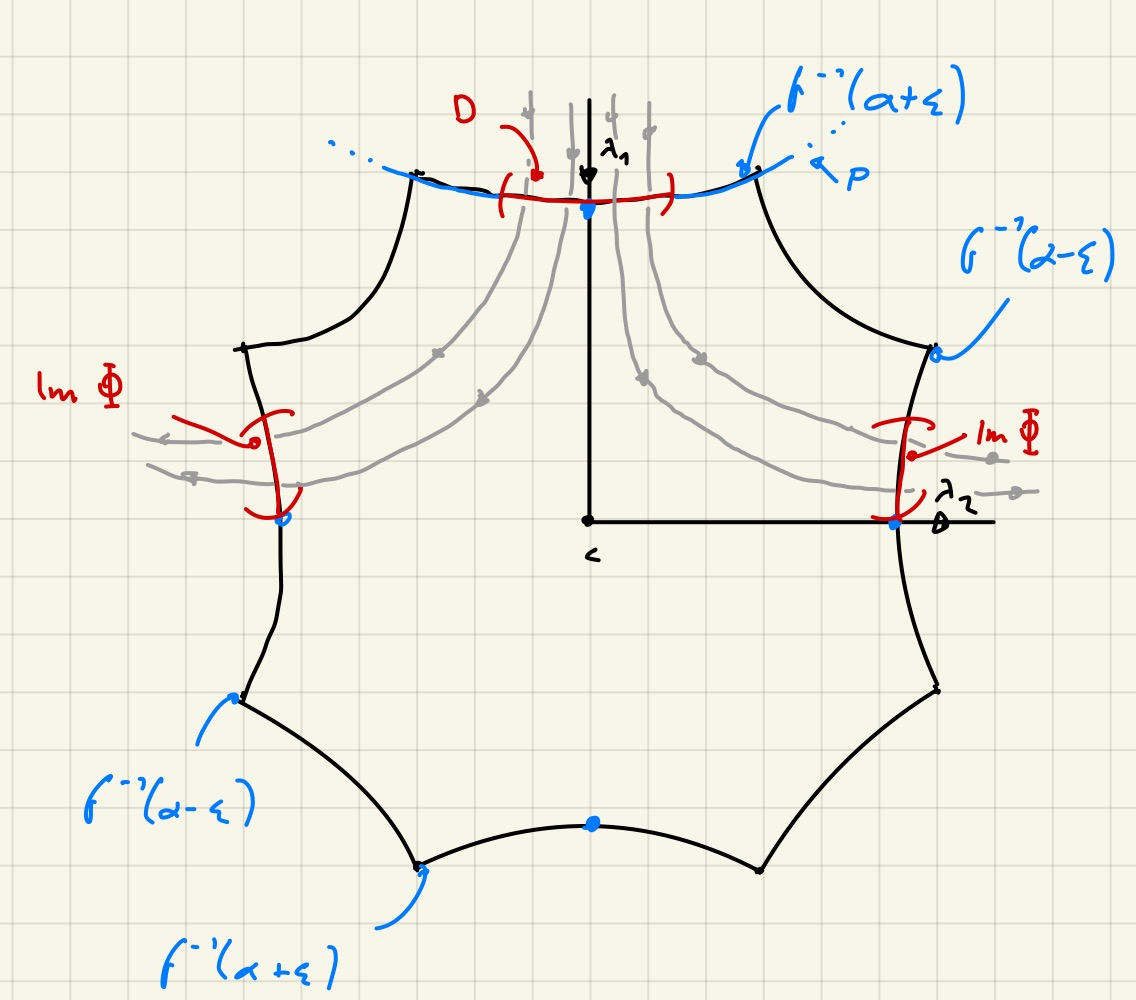
\includegraphics[width=.85\linewidth]{../resources/bew-gebrochene-trajektorien-sind-1-dim-mannigfaltigkeit-2.JPG}
          \captionof{figure}{Another figure}
          \label{fig: test2}
        \end{minipage}
    \end{figure}

    \todo{Zeichnung}

    Man betrachte die Abbildungen~\ref{fig: test1} und~\ref{fig: test2}.

    Wir versuchen, Menge $D - a_1$ entlang der Trajektorien von $X$ auf $\del_- \Omega(c)$ via einer 
    Abbildung $\Phi$ zu projizieren. Wir werden sehen, dass $Q = \Ima (\Phi) \cup S_+(c)$ eine 
    Mannigfaltigkeit mit Rand ist, und dass dann $Q \cap \stab (q)$ eine $1$-dimensionale
    Mannigfaltigkeit mit Rand ist, und $a_2 \in \del q$. Wie in~\ref{prop: wohldefiniertheit von Lt} 
    ist $Q \cap \stab (q) - a_2$ eine Teilmenge von $\Lt (p, q)$, und $a_2 \in \Lt (c, q)$, 
    wenn wir also $a_2 \in \lambda_2$ mit $(\lambda_1, \lambda_2)$ identifizieren, dann bekommen 
    wir unsere Parametrisierung $\psi$ von $\Lb (p, q)$. 
    Also:

    \begin{claim}
        Es sei $\phi$ die von $X$ erzeugfte 1-Parameter Gruppe aus Diffeomorphismen. Für jedes 
        $x \in D - a_1$ existiert ein $t_x \in \R$, sodass $\phi_{t_x} (x) \in \del_- \Omega (c)$
        und $x \mapsto t_x$ glatt ist.
    \end{claim}

    \begin{smallproof}
        Via unserer anfangs gewählten Morse Karte $(V, \kappa)$, und da wir ohne Einschränkungen $D$ 
        klein genug wählen können, sodass $D \subseteq \Omega (c)$, können wir annehmen, dass sich 
        alles im $\R^n$ abspielt ; Sei also ohne Beschränkung der Allgemeinheit 
        $f(x_-, x_+) = - \|x_-\| + \|x_+\|$. Dann ist $\phi$ gegeben durch 
        \[ \phi_t(x_-, x_+) = (e^{2t}x_-, e^{-2t}x_+) . \]
        Falls $(x_-, x_+) \in \del_+ U$ und $x_- \neq 0$, dann gilt auch $x_+ \neq 0$. Setze
        \[ t_{(x_-, x_+)} = \frac{1}{2} \ln \left( \frac{\| x_+ \|}{\| x_- \|} \right) . \]
        Dann gilt
        \[ \phi_{t_{(x_-, x_+)}} (x_-, x_+) = 
            \left( \frac{\| x_+ \|}{\| x_- \|} x_-, \frac{\| x_- \|}{\| x_+ \|} x_+ \right) . \]
        Die Zuordnung $(x_-, x_+) \mapsto t_{(x_-, x_+)}$ ist glatt und 
        \begin{align*}
            f(\phi_{t_{(x_-, x_+)}})(x_-, x_+) = & - \| \frac{\| x_+ \|}{\| x_- \|} x_- \|
                +  \| \frac{\| x_- \|}{\| x_+ \|} x_+ \| \\
                = & - \| x_+ \| + \| x_- \| \\
                = & - \eps .
        \end{align*}
        Es folgt $\phi_{t_{(x_-, x_+)}} (x) \in \del_- U$.
    \end{smallproof}

    Wir haben nun also eine Einbettung $\Phi$ von $D - a_1$ entlang der Trajektorien von $X$ gefunden.
    Wie am Anfang besprochen wollen wir jetzt zeigen:

    \begin{claim}
        Ist $\delta$ klein genug, dann ist $Q = \Phi (D - a_1) \cup S_+ (c)$ eine $k$ dimensionale 
        Mannigfaltigkeit mit Rand, und es gilt $\del Q = S_- (c)$.
    \end{claim}

    \begin{smallproof}
        Wieder spielt sich alles via $\kappa$ im $\R^n$ ab.
        Man betrachte die Projektion
        \[ \pi \colon \R^k \times \R^{n - k} ; \pi (x_-, x_+) = x_- . \]
        und ihre Einschränkung $\del_+ U \to D_{\eta}^k$.
        \todo{weiß net ob das stimmt, naja} Da $S_+ := \kappa(S_+(c)) = (\pi|_{\del_+U})^{-1}(0)$
        und $D \pitchfork S_+$, ist $0$ ein regulärer Wert von $\pi|_{\del_+U}$.
        Also ist $\opd \pi|_{\del_+U} (0)$ surjektiv, und da dim $\del_+U = k = \dim D^k_{\delta}$ ist
        das Differential auch invertierbar. Jetzt können wir den Satz über die Umkehrfunktion anwenden 
        bekommen lokal ein Inverses der Abbildung $\pi|_{\del_+U}$. Es existiert also ein 
        $\delta' \leq \eta$, sodass das Inverse von $\pi|_{\del_+U}$ auf $D^k_{\delta'}$ definiert 
        ist. Dann ist 
        \begin{align*}
            (\pi|_{\del_+U})^{-1} \colon D^k_{\delta'} \longto & D \\
            x_- \longmapsto & (x_-, x_+) =: (x_-, h(x_-))
        \end{align*}
        ein Diffeomorphismus. Da $D \subseteq \del_+U \subseteq f^{-1}(\eps)$, gilt dann 
        $\| h(x_-) \|^2 = \| x_- \|^2 + \eps $. Ist dann 
        $g = \cfrac{h}{\| h \|} \colon D^k_{\delta'} \to S^{n - k - 1}$, dann gilt
        \[ D = \{ (x_-, h(x_-)): x \in D^k_{\delta'} \} 
            = \{ (x_-, \sqrt{\| x_- \|^2 + \eps} \cdot g(x_-)): x \in D^k_{\delta'} \} . \]
        Dann bekommen wir mit der Einbettung aus Behauptung 1 und da $\| g(x_-) \| = 1$:
        \[ \Phi(D - a_1) = 
            \left\{ \left( \frac{\sqrt{\| x_- \|^2 + \eps}}{\| x_- \|} \, x_-, \; 
                    \| x_- \| \, g(x_-) \right) : 
                x_- \in D^k_{\delta'} - 0 \right\} \]
        Wir können nun auf $D^k_{\delta'} - 0$ Polarkoordinaten anwenden. wir erhalten eine 
        Einbettung
        \begin{align*}
            H = \Phi^{-1} \circ \rho \colon (0, \delta') \times S^{k-1} \longto & \del_- U \\
            (r, v) \longmapsto & ( \sqrt{r^2 + \eps} \cdot v, r \cdot g(\rho(r, v))) .
        \end{align*}
        $g$ ist auf ganz $D^k_{\delta'}$ definiert, und wenigstens in einer Umgebung von $0$ 
        beschränkt. Also können wir $H$ stetig in $0$ durch
        \[ H(0, v) = (\sqrt{\eps} \cdot v, \, 0) \]
        fortsetzen. Dann ist $H$ auch weiterhin eine (topologische) Einbettung mit 
        $\Ima (H) = \Phi(D - a_1) \cup S_- $, und es gilt 
        \[ H(0, S^{k - 1}) = S_- . \]
    \end{smallproof}

    Wir wissen, dass für $f(q) < \alpha - \eps < f(c)$ gilt 
    $\Lt (c, q) \diffeo (\unst (c) \cap \stab (q)) \cap f^{-1}(\alpha - \eps)$. 
    
    Außerdem gilt $\stab (q) \pitchfork \Ima \Phi$ und $\stab (q) \pitchfork S_-(c)$ in 
    $f^{-1}(\alpha - \eps)$, also ist mit 
    Proposition~\ref{prop: schnitt von transversalen untermannigfaltigkeiten}
    $\stab (q) \cap Q$ eine Mannigfaltigkeit mit Rand der Dimension $(n - (k - 1)) + k - n = 1$,
    und der Rand von $\stab (q) \cap Q$ ist $\stab (q) \cap S_-(c) \subseteq \Lt (c, q)$, also ist 
    $a_2 \in \del (\stab(q) \cap Q)$.

    Wähle eine Parametrisierung von einer Umgebung von $a_2$ in $\stab (q) \cap Q$
    \[ \chi \colon [0, \delta) \to \stab (q) \cap Q . \]
    Es gilt dann $\chi(0) = a_2$.
    
    Damit erhalten wir die Abbildung 
    \[ \Phi^{-1} \circ \chi \colon (0, \delta) \longto \stab (q) \cap (D - a_1) \subseteq \Lt (p, q) . \]
    Definiere nun 
    \begin{align*} 
        \psi \colon [0, \delta) \longto & \Lb (p, q) \\
        t \longmapsto & \begin{cases}
            \Phi^{-1} \circ \chi (t) & \text{ falls } t \neq 0 \\
            (\lambda_1, \lambda_2) & \text{ falls } t = 0
        \end{cases}
    \end{align*}
    Wir wollen zeigen, dass $\psi$ die gewünschten Eigenschaften vom Anfang erfüllt.

    Offensichtlich ist $\psi$ bijektiv. $\psi$ ist stetig, denn ist $(x_n)_n$ eine Folge in 
    $(0, \delta)$, die gegen $0$ konvergiert, dann konvergiert die Folge $(\chi(x_n))_n$ in 
    $\stab (q) \cap Q \subseteq \del_- \Omega (c)$ gegen $a_2$. Dann folgt aus dem 
    Lemma~\ref{lemma: konvergenz einer folge}, dass die  Folge $(y_n)_n$ in $\stab (q) \cap (D - a_1)$
    mit $y_n = \Phi^{-1}(\chi(x_n))$ gegen $a_1$ konvergiert, also konvergiert $\psi(x_n)$ gegen
    $(\lambda_1, \lambda_2)$. Genau dasselbe gilt für die Umkehrabbildung:

    Ist $(x_n)_n$ eine Folge in $\stab (q) \cap D$, die gegen $a_1$ konvergiert, dann konvergiert
    $\Phi (x_n)$ gegen $a_2$, also $\chi^{-1} (\Phi(x_n))$ gegen $0$.
    Also ist die Abbildung $\psi$ ein Homeomorphismus, und die drei Bedingungen, die an $\psi$ gestellt
    werden, sind offensichtlich aufgrund der Konstruktion erfüllt. 

    Wir müssen nur noch 4. zeigen.

    Sei $(\ell_n)_n$ eine Folge in $\Lt (p, q)$, die gegen $(\lambda_1, \lambda_2)$ konvergiert. 
    Für $n$ groß genug können wir annehmen, dass die $\ell_n$ die Morse Umgebung $\Omega (c)$ betreten 
    und verlassen. Seien wieder wie vorher die $\ell_n^+ = \ell_n \cap \del_+ \Omega (c)$ die Punkte, 
    an denen $\ell_n$ die Umgebung $\Omega (c)$ verlässt und $\ell_n^- = \ell_n \cap \del_- \Omega (c)$
    die Punkte, an denen $\ell_n$ in die Umgebung $\Omega (c)$ eintritt. Wegen der Topologie, die wir 
    auf $\Lb(p, q)$ definiert haben gilt offensichtlich
    \[ \lim_{n \to \infty} \ell_n^- = a_1 \; \; \text{ und } \; \; \lim_{n \to \infty} \ell_n^+ = a_2 , \]
    und da $\Phi$ den Trajektorien von $X$ folgt gilt $\Phi(\ell_n^-) = \ell_n^+$.
    Für $n$ groß genug gilt also $\ell_n^- \in D - a_1$, also $\ell_n^+ \in Q$. Sowieso gilt schon, dass
    $\ell_n^+ \in \stab (q)$, also 
    \[ \ell_n^- \in Q \cap \stab (q) = \Ima \chi . \]
    Außerdem ist $\Phi^{-1}(\ell_n^+) = \ell_n^-$, also $\ell_n \in \Ima (\psi)$.
\end{bigproof}

\subsection*{Der Morse Komplex über \texorpdfstring{$\Z$}{TEXT}}

Wir haben nun den Morse Komplex über $\F_2$ definiert. Wir wollen noch allgemeiner einen Komplex
über $\Z$ definieren. Die meiste Arbeit dafür ist nun schon gemacht. Um den Morse-Komplex über 
$\Z$ zu definieren, wollen wir den Raum der Trajektorien $\Lt (p, q)$ orientieren. Dafür beschäftigen 
wir uns ein wenig mit Orientierungen von Vektorräumen.

\begin{definition}[Orientierung und Koorientierung]
    Es sei $V$ ein endlich dimensionaler Vektorraum. Seien außerdem $\B_1$ und $\B_2$ Basen von $V$. 
    Definiere
    \[ \B_1 \sim_O \B_2 \Longleftrightarrow \det \, _{\B_1}[\id_V]_{B_2} > 0 \]
    Man rechnet leicht nach dass $\sim_O$ eine Äquivalenzrelation ist und dass es bezüglich $\sim_O$
    genau zwei Äquivalenzklassen gibt.
    Zwei Basen heißen \textit{gleich orientiert} wenn sie äquivalent bezüglich $\sim_O$ sind. 
    Eine \textit{Orientierung} ist eine Wahl der Äquivalenzklasse. Ein \textit{orientierter Vektorraum} 
    ist ein Vektorraum zusammen mit einer Orientierung. Ist ein Vektorraum orientiert, dann sagen wir 
    dass eine Basis \textit{positiv orientiert} ist, falls sie gleich orientiert mit der gewählten Basis 
    ist.

    Sei nun $U$ ein Unterraum von $V$ und $\B_0$ eine Basis von $U$. Sind $\B_1$ und $\B_2$ Basen von 
    zwei (möglicherweise verschiedenen) Komplementärräumen von $U$, dann definiere
    \[ \B_1 \sim_K \B_2 \Longleftrightarrow \det \, _{(\B_1, \B_0)}[\id_V]_{(\B_2, \B_0)} > 0 . \]
    Man rechnet leicht nach, dass $\sim_K$ eine Äquivalenzrelation ist, dass es bezüglich $\sim_K$
    genau zwei äquivalenzklassen gibt, und dass $\sim_K$ nicht von der gewählten Basis $\B_0$ abhängt. 
    Zwei Basen heißen \textit{gleich koorientiert} wenn sie äquivalent sind. Eine \textit{Koorientierung} 
    von $U$ ist eine Wahl der Äquivalenzklasse. Ein \textit{koorientierter Vektorraum} ist ein Vektorraum 
    zusammen mit einer Koorientierung. Ist ein Vektorraum koorientiert, dann sagen wir dass eine Basis 
    eines Komplements von $U$ \textit{positiv koorientiert} ist, falls sie gleich koorientiert mit der 
    gewählten Basis ist.
\end{definition}

\begin{prop}
    Es seien $U, W \subseteq V$ Untervektorräume, $U$ orientiert und $W$ koorientiert. Dann ist 
    $U \cap W$ orientiert.
\end{prop}

\begin{proof}
    Wähle eine Basis $\B$ von $U \cap W$. Erweitere $\B$ mit einer positiv koorientierten Basis $\B_1$
    bezüglich $W$ zu einer Basis von $U$. Dann ist $\B$ positiv orientiert, falls $(\B_1, \B)$ 
    in $U$ positiv orientiert ist. Dies hängt nicht von der Wahl von $\B_1$ ab:

    Sei $\B_2$ eine weitere positiv koorientierte Basis eines Komplements von $W$, sodass $(\B_2, \B)$ 
    eine Basis von $U$ mit derserlben Orientierung wie $(B_1, \B)$ ist. Sei $\tilde{\B}$ gewählt, sodass 
    $(B, \tilde{\B})$ eine Basis von $W$ ist. Dann sind $(\B_1, \B, \tilde{\B})$ und 
    $(\B_2, \B, \tilde{\B})$ Basen von $V$, und es gilt
    \[ 0 < \det \, _{(\B_1, \B, \tilde{\B})}[\id_V]_{(\B_2, \B, \tilde{\B})} = 
        \det \, _{(\B_1, \B)}[\id_U]_{(\B_2, \B)} \]
\end{proof}

\begin{definition}[Orientierung und Koorientierung von Mannigfaltigkeiten]
    Es sei $M$ eine $n$-dimensionalen Mannigfaltigkeit und 
    \[ (v_1, \dots, v_n), (w_1, \dots, w_n) \colon M \to TM \times \dots \times TM \]
    glatte Abbildungen mit $v_i(p), w_i(p) \in T_pM$, für alle $p \in M$ sodass $(v_1(p), \dots, v_n(p))$
    und $(w_1(p), \dots w_n(p))$ Basen von $T_pM$ sind. Dann definiere:
    \[ (v_1, \dots, v_n) \sim_O (w_1, \dots, w_n) 
        \Longleftrightarrow 
            (v_1(p), \dots, v_n(p)) \sim_O (w_1(p), \dots, w_n(p)) \text{ für alle } p \in M . \]
    Dies ist wieder eine Äquivalenzrelation und es gibt wieder genau zwei Äquivalenzklassen. 
    Eine Äquivalenzk
\end{definition}

Die stabilen Mannigfaltigkeiten sind offene Kreisscheiben, also offensichtlich orientierbar. 
Wähle für jeden kritischen Punkt $p$ (endgültig) eine Orientierung von $\stab (p)$. Da gilt 
$T_p \stab (p) + T_p \unst (p) = T_p M$ und $\dim T_p \stab (p) + \dim T_p \unst(p) = n$,
gilt schon $T_p \stab (p) \oplus T_p \unst (p) = T_p M$. Die Wahl der Orientierung von $\stab (p)$
ist also gleichzeitig eine Wahl der Koorientierung von $\unst (p)$. Dann ist für kritische Punkte 
$\stab (p) \cap \unst (p)$ eine orientierte Mannigfaltigkeit. 

Bemerke nun, dass fur einen regulären Wert $c$ die Niveau-Menge $f^{-1}(c)$ transversal zum 
Pseudo-Gradientenfeld $X$ liegt, und da $f^{-1}(c)$ $n-1$-dimensional ist definiert $X$ eine 
Koorientierung von $f^{-1}(c)$. Außerdem gilt für reguläre Werte mit $f(p) > c > f(q)$, dass 
$\Lt (p, q) = (\unst (p) \cap \stab (q)) \cap f^{-1}(c)$. Also ist $\Lt (p, q)$ orientiert.

Falls nun $p$ und $q$ kritische Punkte mit $\Index (p) = \Index (q) + 1$ sind, dann ist wieder 
$\Lt (p, q)$ nur eine Ansammlung von Punkten, die alle mittels der Orientierung mit einem Vorzeichen 
ausgestattet wurden. Es sei $N_X (p, q)$ die Summe dieser Vorzeichen. Dann sei $C_k (M, (f, X))$
das von den kritischen Punkten von $f$ mit Index $k$ erzeugte $\Z$-Modul, und für einen kritischen $p$
sei
\[\del_X (p) = \sum_{\substack{ q \in \Crit(f) \\ \Index (p) + 1 = \Index (q) }} N_X(p, q)p . \]

Wir müssen nun dieselben Fragen beantworten wie für den Komplex über $\F_2$. 

Offensichtlich ist $N_X(p, q) < \infty$. Wir müssen also noch zeigen, dass gilt
\[ \del_X \circ \del_X (p) = 0 . \]
Dies folgt aus dem Satz~\ref{satz: gebrochene trajektorien sind 1-dim mannigfaltigkeit}.
Die Kompaktifizierung einer orientierten \\ 
$1$-dimensionalen Mannigfaltigkeit zu einer $1$-dimensionalen 
Mannigfaltigkeit mit Rand ist offensichtlich wieder orientiert. Wir müssen nur noch sicherstellen, dass 
die Orientierung auf dem Rand dann auch mit der Orientierung, die wir oben festgelegt haben übereinstimmt.



\chapter{Morse-Homologie und zelluläre Homologie}

In diesem Kapitel wird aus einem Morse-Smale Paar auf einer Mannigfaltigkeit
eine zelluläre Struktur dieser Mannigfaltigkeit konstruiert. Dann werden wir 
sehen, dass der Kettenkomplex, der von dieser Struktur induziert wird schon mit
dem Morse-Komplex übereinstimmt. Somit stimmt die Morse-Homologie mit der 
zellulären Homologie überein, also auch mit der singulären Homologie.

\section{CW-Komplexe}

\begin{definition}[CW-Komplex]
    \label{def: cw-komplex}

\end{definition}

\begin{definition}[Zellulärer Kettenkomplex]
    \label{def: zellulärer Kettenkomplex}

\end{definition}
\section{CW-Struktur von Mannigfaltigkeiten}
\section{Morse-Homologie ist zelluläre Homologie}
\section{Anwendungen}

\appendix

\chapter{Anhang}

\begin{definition}[Mannigfaltigkeit \cite{ludwig}]
    \label{anh.def: mannigfaltigkeit}
    Es sei $M$ ein topologischer Raum. 
    
    Eine \textit{Karte} von $M$ ist ein Tupel
    $(U, \phi)$, wobei $U \subseteq M$ offen und $\phi \colon U \to U' \in \R^n$ 
    ein Homeomorphismus ist.

    $\mathcal{A} = \left\{ (U_{\alpha}, \phi_{\alpha}) \right\}_{\alpha \in I}$ ist ein 
    \textit{$n$-dimensionaler Atlas} von $M$ falls
    \begin{enumerate}
        \item $(U_{\alpha}, \phi_{\alpha})$ ist eine Karte für jedes $\alpha \in I$
        \item $M = \bigcup_{\alpha \in I U_{\alpha}}$
    \end{enumerate}
    Ein Atlas ist $C^k$ für $k \in \{ \N_0 \cup \{ \infty, \omega \} \}$, falls für
    alle $\alpha, \beta \in I$ der \textit{Koordinatenwechsel} 
    \[ 
        \phi_{\alpha \beta} := 
        \phi_{\alpha} \circ \phi_{\beta}^{-1} \colon 
        \phi_{\beta} (U_{\alpha} \cap U_{\beta}) \to \phi_{\alpha} (U_{\alpha} \cap U_{\beta})
    \]
    $C^k$ ist.
    
    Eine Karte $(U, \phi)$ heißt \textit{$C^k$ kompatibel} mit einem $C^k$ Atlas 
    $\mathcal{A} = \left\{ (U_{\alpha}, \phi_{\alpha}) \right\}_{\alpha \in I}$,
    falls für alle $\alpha \in I$ die Koordinatenwechsel $\phi \circ \phi_{\alpha}^{-1}$
    und $\phi_{\alpha} \circ \phi^{-1}$ $C^k$ sind.

    Eine \textit{$n$-dimensionale $C^k$ Mannigfaltigkeit} ist ein topologischer Raum $M$ 
    zusammen mit einem maximalen $C^k$ Atlas $\mathcal{A}$, sodass $M$ ein Hausdorff-Raum und
    zweitabzählbar ist. Maximal bedeutet hier, dass es keine mit $\mathcal{A}$ $C^k$ 
    kompatiblen Karten gibt, die nicht in $\mathcal{A}$ enthalten sind.

    Eine Mannigfaltigkeit heißt \textit{glatt} falls $k = \infty$.

    Für einen Punkt $p \in M$ und eine Karte $(\phi, U)$ mit $p \in U$ 
    heißen $\phi = (x_1, ..., x_n)$ \textit{lokale Koordinaten} um $p$.
\end{definition}

\begin{remark}
    Wenn der Atlas einer Mannigfaltigkeit angegeben wird, dann nie als maximaler Atlas.
    Es reicht ein Atlas, alle anderen Karten sind dann schon impliziert.
\end{remark}

\begin{definition}[Differenzierbarkeit]
    \label{anh.def: differenzierbarkeit}
    Sind $M, N$ $C^k$ Mannigfaltigkeiten, \\ 
    $\mathcal{A} = (\phi_{\alpha}, U_{\alpha})_{\alpha \in I}$ ein Atlas von $M$, 
    $\mathcal{B} = (\phi_{\beta}, U_{\beta})_{\beta \in J}$ ein Atlas von $N$,
    dann heißt eine Abbildung $C^k$ oder \textit{$k$-mal differenzierbar}, falls für alle 
    $\alpha \in I$ und $\beta \in J$ die Abbildung
    \[ \psi_{\beta} \circ f \circ \phi_{\alpha}^{-1} \colon \R^n \to \R^m \]
    $C^k$ ist.
\end{definition}

\begin{definition}[Tangentialraum]
    \label{anh.def: tangentialraum}
    Der Tangentialraum einer $C^k$ Mannigfaltigkeit $M$ an einem Punkt $p \in M$ ist
    \[ T_pM := \left\{ X_p \colon C^{k} \to \R : X_p 
        \text{ ist eine Derivation von $M$ an dem Punkt $p$} \right\} \]
    Wobei $X_p: C^{k} \to \R$ ein \textit{Derivation} ist, falls folgende Bedingungen erfüllt
    sind:
    \begin{itemize}
        \item $X_p$ ist linear
        \item Für $X_p$ gilt die Leibnitz-Regel, also
            \[ X_p (f \cdot g) = X_p (f) \cdot g + f \cdot X_p (g) \]
    \end{itemize}
    Dann ist $T_pM$ ein Untervektorraum von $C^k(C^k(M))$.

    Für eine $C^k$ Abbildung $f \colon M \to N$  und einen Punkt $p \in M$ ist dann 
    \begin{align*}
        \opd f (p) \colon T_pM & \to T_{f(p)}N \\
        X_p & \mapsto f_* X_p
    \end{align*}
    wobei $f_*X_p$ definiert ist durch
    \[ f_*X_p (g) = X_p (g \circ f) \]
\end{definition}

\begin{remark}
    \begin{align*}
        T \colon \mathbf{Man}_{*} & \to \mathbf{Vect}_{\R} \\
        (M, p) & \mapsto T_pM \\
        f & \mapsto \opd f (p)
    \end{align*}
    Ist ein Funktor.
\end{remark}

\begin{remark}
    Es sei $M$ eine $C^k$ Mannigfaltigkeit, $k \geq 1$, $p \in M$ und $\phi = (x_1, ..., x_n)$
    lokale Koordinaten um $p$. Definiere
    \begin{align*} 
        \pderive{x_1}(p): C^k(M) & \to \R \\
        \pderive[f]{x_i} (p) & = \pderive[\phi \circ f]{x_i} (\phi(p))
    \end{align*}
    Dann ist $\left( \pderive{x_i} \right)_{1 \leq i \leq n}$ eine Basis von $T_pM$.

    Für eine glatte Abbildung $f \colon M \to N$, einem Punkt $p \in M$ und lokale Koordinaten 
    $(x_1, ..., x_n)$ um $p$ und $(y_1, ..., y_m)$ um $f(p)$ bekommen wir in einer Umgebung 
    von $p$ wohldefinierte Abbildungen $f_i = y_i \circ f$. Dann ist das differential 
    $\opd f (p)$ von $f$ gegeben durch die Matrix
    \[ D_p(f) = \left( \pderive[f_i]{x_j} \right)_{i,j} . \]
\end{remark}

\begin{definition}
    \label{anh.def: kritischer punkt}
    Es seien $M, N$ $C^k$ Mannigfaltigkeiten. Sei $f \colon M \to N$ $C^k$. Dann ist $p \in M$
    ein kritischer Punkt von $f$, falls $\opd f (p)$ nicht surjektiv ist. $f(p)$ heißt dann
    kritischer Wert von $f$.
\end{definition}

\begin{theorem}[Whitney's Einbettungssatz, \cite{hirsch}]
    \label{anh.satz: whitneys einbettungssatz}
    Es sei $M$ eine $n$-dimensionale kompakte \todo{Finde eine Quelle ohne Kompaktheit} 
    $C^r$ Mannigfaltigkeit. Dann existiert eine $C^r$ Einbettung von $M$ in 
    $\R^{2n + 1}$.
\end{theorem}

\begin{remark}
    Man kann zeigen, dass jede Mannigfaltigkeit sogar in den $\R^{2n}$ eingebettet werden.
    Diese Version des Satzes heißt \textit{starker Whitney's Einbettungssatz}.
\end{remark}

\begin{theorem}[Satz von Sard (siehe \cite{sard})]
    \label{satz: satz von sard}
    Es seien $M$ und $N$ mindestens \\ 
    $C^q$-Mannigfaltigkeiten mit Dimension $m$ und $n$ respektive
    und $f \colon : \to N$ mindestens $C^q$. Dann gelten:
    \begin{itemize}
        \item Falls $m \leq n$, dann hat die Menge der kritischen Werte von $f$ Maß $0$.
        \item Falls $m > n$, dann hat die Menge der kritischen Werte von $f$ Maß $0$, \\
            falls $q \geq m - n + 1$.
    \end{itemize}
\end{theorem}


\printbibliography

\eject
\end{document}